\documentclass[thesis=B,czech]{FITthesis}[2012/06/26]

\usepackage[utf8]{inputenc} % LaTeX source encoded as UTF-8

\usepackage{graphicx} %graphics files inclusion
\usepackage{amsmath} %advanced maths
% \usepackage{amssymb} %additional math symbols
\usepackage[figuresleft]{rotating}
\usepackage[flushleft]{threeparttable} % for footnote in tabular
\usepackage{fancyvrb}
\usepackage{microtype}

\usepackage{dirtree} %directory tree visualisation

\usepackage{enumitem}
\setlist[enumerate]{label*=\arabic*.}

% % list of acronyms
% \usepackage[acronym,nonumberlist,toc,numberedsection=autolabel]{glossaries}
% \iflanguage{czech}{\renewcommand*{\acronymname}{Seznam pou{\v z}it{\' y}ch zkratek}}{}
% \makeglossaries

\newcommand{\tg}{\mathop{\mathrm{tg}}} %cesky tangens
\newcommand{\cotg}{\mathop{\mathrm{cotg}}} %cesky cotangens

% ______ MACROS ___________________________________________________________
% Macros to use as research features criteria. 
% The text is used repeatedly, so in case of its change I want the change
% to happen everywhere.
\newcommand{\crita}{Nevyžaduje vlastní infrastrukturu, rychlé zprovoznění}
\newcommand{\critb}{Použitelnost}
\newcommand{\critc}{Absence nepotřebné funkcionality}
\newcommand{\critd}{Použití zdarma}
\newcommand{\crite}{Funkce}
\newcommand{\critf}{REST API}
\newcommand{\critg}{Open source}


\newcommand{\forwatchers}{Povoleno jen pro Pozorovatele úkolu.}
\newcommand{\forworkers}{Povoleno jen pro Pracovníky úkolu.}
\newcommand{\foradmin}{Povoleno jen pro Admina skupiny.}
\newcommand{\formanagers}{Povoleno jen pro Manažery skupiny.}
\newcommand{\formembers}{Povoleno jen pro Členy skupiny.}
% _________________________________________________________________________


\department{Katedra Softwarového Inženýrství}
\title{Systém správy úkolů pro jednotlivce a malé týmy}
\authorGN{Martin} %(křestní) jméno (jména) autora
\authorFN{Melka} %příjmení autora
\authorWithDegrees{Martin Melka} %jméno autora včetně současných akademických titulů
\supervisor{Ing. Josef Pavlíček, Ph.D.}
\acknowledgements{Doplňte, máte-li komu a za co děkovat. V~opačném případě úplně odstraňte tento příkaz.}

\abstractCS{Tato bakalářská práce se zabývá srovnáním existujících aplikací a tvorbou nové aplikace pro správu úkolů. Uživateli této aplikace budou jednotlivci a menší pracovní skupiny, které chtějí přidělovat zodpovědnosti a sledovat průběh práce na společných úkolech. Aplikace umožní lidem sdružovat se do skupin, spolupracovat na sdílených úkolech a zaznamenávat odvedenou práci. Součástí této práce je definice požadavků na aplikaci, srovnání navrhovaného řešení s existujícími aplikacemi, dále návrh, implementace, testování a nasazení aplikace. Výsledkem práce bude aplikační backend, vystavující funkcionalitu skrze REST rozhraní.}

\abstractEN{The aim of this thesis is to compare available software applications for task management and to subsequently create an original one. The users of this application will be individuals and small-scale workgroups, who need to assign responsibilities for and track the progress of shared tasks. The application will allow users to form groups, work together on shared tasks and report the work done on them. This thesis consists of a definition of application requirements, comparison of current task management solutions and design, implementation, testing and deployment of the proposed application. The outcome of this thesis will be an application backend, which exposes its functionality through a REST interface.}
\placeForDeclarationOfAuthenticity{V~Praze}
\declarationOfAuthenticityOption{4} %volba Prohlášení (číslo 1-6)
\keywordsCS{Správa úkolů, produktivita, organizace týmů, backend, REST, Java Spring Framework}
\keywordsEN{Task management, productivity, team organization, backend, REST, Java Spring Framework}

\begin{document}

% \newacronym{CVUT}{{\v C}VUT}{{\v C}esk{\' e} vysok{\' e} u{\v c}en{\' i} technick{\' e} v Praze}
% \newacronym{FIT}{FIT}{Fakulta informa{\v c}n{\' i}ch technologi{\' i}}

\begin{introduction}
	Výpočetní technika umožnila rozvoj rychlejší a efektivnější komunikace, práce a vůbec způsobu života. Je běžné mít svůj kalendář on-line a sdílet ho s ostatními, případně používat některý nástroj s funkcí úkolníčku. Zejména ve velkých firmách, kde existuje silná potřeba koordinovat úsilí mnoha lidí, tak vznikla poptávka po nástrojích pro správu úkolů, které by jim umožnily efektivnější rozdělování zodpovědností a práce. Řešení, které na tento popud vznikly, slouží právě potřebám velkých firem. Potřeby menších skupin a jednotlivců jsou ale jiné. Pro ně jsou tyto nástroje příliš komplexní, těžkopádné a nedostatečně intuitivní.

	Tato práce se zabývá přehledem existujících řešení pro správu úkolů malých i velkých skupin a tvorbou backendu nové aplikace. Aplikace bude zaměřena na potřeby menších týmů a jednotlivců a bude umožňovat uživatelům vytvářet úkoly, sdílet je s ostatními uživateli, sdružovat se do skupin a zaznamenávat průběh práce na úkolech. 
	
	V první části porovnám současná řešení pro správu úkolů z pohledu malých týmů a jednotlivců. 
	
	Ve druhé části se zabývám analýzou problému. Definuji požadavky na aplikaci ve formě uživatelských příběhů a podrobím je analýze.
	
	Ve třetí části vypracuji návrh řešení aplikace. Zde vybírám technologii pro implementaci a popisuji architekturu aplikace, návrhový model tříd a databázový model.
	
	Ve čtvrté části popisuji implementaci aplikace.
	
	V páté části se věnuji testování aplikace za účelem zjištění její správné funkčnosti. Popíšu zde použité technologie a způsob testování.
	
	V poslední, šesté části, vysvětlím, jak výslednou aplikaci nasadit a spustit.
\end{introduction}

%%%%%%%%%%%%%%%%%%%%%%%%%%%%%%%%%%%%%%%%%%%%%%%%%%%%%%%%%%%%%%%%%%%%%%%%%%%%%%%%%%%%%%%%%%%%%%%%%%%%%%%%%
%%%%%%%%%%%%%%%%%%%%%%%%%%%%%%%%%%%%%%%%%%%%%%%%%%%%%%%%%%%%%%%%%%%%%%%%%%%%%%%%%%%%%%%%%%%%%%%%%%%%%%%%%
\chapter{Slovník pojmů}
	\begin{description}
		\item[Deadline] je časová lhůta, do které je nutné dokončit nějakou práci. Jeho synonyma jsou uzávěrka a konečný termín.
		
		\item[Assignee] je člověk přidělený k určitému úkolu, je zodpovědný za práci na něm.
		\item[Open source software] je softwarové dílo, k němuž jsou veřejně dostupné jeho zdrojové kódy.
		\item[Gamifikace] je uplatňování technik z herního designu a herních principů do neherních oblastí. Slouží například k motivaci formou získávání bodů za určité činnosti a zobrazováním grafů jejich vývoje.
		\item[Backend] je část webové aplikace, která nekomunikuje přímo s uživatelem. V kontextu této práce zprostředkovává aplikační logiku a s okolím komunikuje skrze definované rozhraní.
		\item[Manhour] je jednotka práce. Jeden člověk odpracuje za hodinu jeden \textit{manhour}. Vypočte se jako: $manhours = lidi \times hodiny$.
		\item[Embedded] znamená vestavěný, zabudovaný. 
	\end{description}
\chapter{Současný stav}
	\label{chapter:current-state}

	Způsobů, jak řešit správu úkolů, existuje spoustu a liší se podle toho, kdo je má využívat. V této části práce představím několik zástupců pro každou ze tří kategorií. Těmi jsou:
	\begin{enumerate}
	  \item řešení pro větší firmy s množstvím pracovníků;
	  \item řešení pro střední a menší týmy, jednotky až desítky pracovníků;
	  \item řešení pro jednotlivce.
	\end{enumerate}

	Zástupce vybírám podle osobních zkušenosti a podle výsledků získaných z vyhledávače \texttt{Google}, na základě jejich pořadí a popularity mezi uživateli. U uvedených zástupců uvedu krátký popis a jejich použitelnost cílovou skupinou této práce, tj. menšími týmy a jednotlivci.

	Pracuji s tím, že pro cílovou skupinu této práce jsou důležitá následující kritéria:
	\begin{enumerate}
		\item \textbf{\crita} -- Uživatelé nechtějí spravovat vlastní hardware, kde by jim aplikace běžela. Začít používat aplikaci má být otázka maximálně několika málo minut.
		\item \textbf{\critb} -- Kritérium jsem hodnotil subjektivně, podle mého názoru na pět kvalitativních částí použitelnosti\cite{usability}. Uživatel by se neměl ztratit ve funkcích aplikace a měl by být schopen rychle pochopit, jak s aplikací pracovat. 
		\item \textbf{\critc} -- 	Aplikace by měla obsahovat jen základní funkce, které uživatel využije. Větší množství funkcí, které uživatele nezajímají, ztěžují orientaci v aplikaci, což souvisí s předchozím bodem.
		\item \textbf{\critd} -- Aplikace by měla být použitelná zdarma. V případě, že se jedná o \textit{freemium} model, měla by její neplacená část stačit k běžnému používání a neomezovat výrazně uživatele.
		\item \textbf{\critf} -- Aplikace by měla nabízet rozhraní REST API pro možnost vlastní integrace na její funkce.
		\item \textbf{\critg} -- Aplikace by měla mít veřejně dostupné zdrojové kódy.
	\end{enumerate}
	Uvedený přehled není vyčerpávající, věnuji se jen některým z těch nejznámějších řešení. 

	\section{Řešení pro firmy}
		\label{sec:solutions-companies}
		Řešení této kategorie se zaměřují na větší počet uživatelů a mimo základní správy úkolů nabízí často další funkce pro řízení projektů a integraci s dalšími systémy. Používají se zejména v oblasti vývoje software, ale dají se využít i v jiných oblastech.
		
		\subsection{JIRA}
			JIRA \cite{jira} je software, který nabízí systém pro řízení požadavků (angl. bug tracking či issue tracking) a funkce pro správu projektů. Je možné ho používat jak na vlastní infrastruktuře, tak on-line. V prvním případě je použití zdarma za určitých podmínek\footnote{Zdarma pro veřejně dostupný open-source software projekt\cite{jira-lic-opensource} a pro neziskové, nevládní, neakademické, nekomerční a sekulární instituce, které by si jinak nemohly software dovolit. \cite{jira-lic-nonprofit}}, v druhém případě je použití placené. 
			
			Nabízí širokou funkcionalitu a např. možnost upravovat podle potřeb životní cyklus úkolů. To ho činí využitelným i mimo vývoj software. Množství nabízených funkcí jde ale nad potřeby cílové skupiny této práce a technicky méně zdatné uživatele může mást. Na úkolech lze pracovat ve více lidech, ale přiřazen může být v jednu chvíli jen jednomu uživateli (\textit{assignee}). Úkolům lze také přiřadit \textit{deadline}.
			
			JIRA nabízí REST API a není open source.
			
		\subsection{Bugzilla}
			Bugzilla \cite{bugzilla} je systém řízení požadavků, který je zaměřen hlavně na vývoj software. Je podobný nástroji JIRA, nicméně nenabízí takovou flexibilitu a i když by mohl být s dobře nastavenou politikou použitý pro správu úkolů u jiných než softwarových projektů, nebylo by použití intuitivní. Samotná správa a práce s úkoly funguje stejně jako u nástroje JIRA.
			
			Bugzilla je open source, licencovaná pod MPL, a lze ji využít zdarma i pro komerční účely. Je nutné ji ale provozovat na vlastním hardware. Existují hosting služby, které jsou ale neoficiální a placené. Bugzilla nabízí REST API.
			
		\subsection{Redmine}		
			Redmine \cite{redmine} je systém řízení požadavků, který nabízí více flexibility než Bugzilla a obsahuje i některé nástroje pro řízení projektů. Tyto nástroje mohou být přínosné pro větší projekty, které mají danou strukturu, ale nepočítám s tím, že by cílovou skupinu této práce zajímaly. Funkcionalita, která se týká správy úkolů, je srovnatelná s předchozími dvěma nástroji.
			
			Použití je zdarma, ale je nutné nainstalovat na vlastním hardware. Stejně jako v případě nástroje Bugzilla není Redmine oficiálně použitelný on-line, soukromé hostingy jsou placené. Projekt je vyvíjen jako open source a nabízí REST API.

	\section{Řešení pro střední a menší týmy}
		\label{sec:solutions-teams}
		Nástroje v této kategorii se snaží cílit na týmy, spíše než celé firmy, a práce s nimi není tak formální. Používat je lze on-line, není nutné vlastní instalace. Oproti řešením v bodu \ref{sec:solutions-companies} obsahují tyto méně funkcí, chybí hlavně různé manažerské nástroje a integrace s dalšími systémy.
	
		\subsection{Trello}
			Trello \cite{trello} je on-line aplikace, která vznikla v roce 2011. Způsob správy úkolů staví na konceptu \textit{kanban}\cite{kanban}. Umožňuje vytvářet nástěnky (boards), které reprezentují projekty. K nástěnkám lze přizvat další uživatele a pracovat na nich společně. Na nástěnkách se dají vytvářet seznamy (lists) a v nich karty (cards), které představují nejmenší jednotku práce - úkol. Ten má svou prioritu, \textit{deadline} a zodpovědné uživatele. Těch může být libovolný počet.
			
			Je to funkčně bohatý nástroj s jednoduchým ovládáním i pro netechnické uživatele. Na profilu uživatele lze zobrazit všechny přiřazené karty a ty seřadit podle nástěnky, kam patří, nebo podle jejich \textit{deadlinu}. 
			
			Trello je možné používat zdarma s libovolným počtem spolupracovníků. Placené varianty přináší určité výhody\cite{trello-pricing}, ale menší týmy se moho obejít bez nich. Existuje i REST API\cite{trello-api}, aplikace není open source.
		
			
		\subsection{Trackie}
			Trackie \cite{trackie} je on-line aplikace, která je určena pro správu úkolů na společných projektech. Ty lze zakládat a zvát do nich uživatele, v rámci projektů pak tvořit úkoly. Úkol může být někomu přiřazen, ale vždy jen jednomu uživateli. Funkčností i vzhledem jednoduché na použití, ale některé funkce oproti předchozím nástrojům chybí. Úkolům například nelze nastavit \textit{deadline}. Zobrazit je možné jen úkoly každého projektu zvlášť, nelze zobrazit přehled všech úkolů uživatele. 
			
			Aplikace nabízí 30denní zkušební dobu, po její uplynutí je placená. Nenabízí REST API a není open source.
			
		\subsection{FogBugz}
			FogBugz \cite{fogbugz} je nástroj řízení projektů, který kromě podpory řízení požadavků nabízí i možnost agilního plánování\cite{agile-planning}, správu podpory a zpětné vazby zákazníků, vytváření dokumentů ve stylu Wiki a další. Nabídkou funkcí je nejbohatší z trojice nástrojů v této kategorii, i přesto se v aplikaci uživatel neztratí. 
			
			Uživatelé spolu mohou pracovat na úkolech (cases), které se dělí do projektů (projects). Na úkolu lze evidovat informace potřebné pro využití agilní metodiky plánování, včetně \textit{story points}. Úkolu je možné určit zodpovědného uživatele, odhad pracnosti a deadline. Na úkolu je možné průběžně zaznamenávat odpracovanou práci a zobrazovat kolik času na něm zbývá.
			
			FogBugz nabízí 7denní zkušební dobu zdarma, poté je nutné za používání platit. Je možné ho používat jak on-line, tak na vlastním hardware. Nabízí REST API a není open source.

	\section{Řešení pro jednotlivce}
		\label{sec:solutions-individuals}
		Poslední kategorií jsou nástroje pro správu úkolů jednotlivců. Některé z nich mohou umožňovat sdílení úkolů, takže by se daly zařadit i do kategorie \ref{sec:solutions-teams}, nicméně svým zaměřením cílí primárně na využití jako osobní úkolníček, proto jsou zařazeny zde. Také jsem do této kategorie zařadil nástroje, které nejsou primárně určeny pro správu úkolů, ale někteří je k tomuto účelu využívají, například kalendář nebo poznámky.
		
		\subsection{Todoist}
			Todoist \cite{todoist} je on-line aplikace pro organizaci úkolů, která má uživatele motivovat k lepší produktivitě. Za splněné úkoly jsou přidělovány body (karma), jejichž historický vývoj je možné sledovat v grafu, lze nastavit denní a týdenní cíl a získávat další \uv{odměny} za jeho splnění. Úkoly lze rozdělit do projektů, nastavit jim \textit{deadline}, prioritu a opakování. Projekty je možné sdílet s dalšími uživateli a dají se zobrazit buď po projektech, ke kterým patří, nebo všechny na jednom místě -- ve schránce (inbox). 
			
			Vytvoření nového úkolu se může provést zadáním (anglického) textu, aplikace sama rozpozná klíčová slova a není tak nutné nastavovat vlastnosti úkolů ručně. Například heslo \textit{Go jogging at 1 PM every day} vytvoří úkol \textit{Go jogging}, který má \textit{deadline} ve 13 hodin a opakuje se každý den. 
			
			Placená verze nabízí větší množství otevřených projektů a úkolů, hledání v úkolech, notifikace a další.\cite{todoist-compare-premium} Todoist nabízí REST API\cite{todoist-api} a není open source.
			
		\subsection{Toodledo}
			Toodledo \cite{toodledo} je on-line aplikace, která kromě úkolů umožňuje vytvářet si zvyky (habits). To jsou úkoly, které se opakují ve volitelné dny každý týden, jež mají uživatelům pomoci vypěstovat si a dodržovat dobré návyky. Po vykonání zvyku je možné označit ho za splněný a přidat k jeho splnění číslo nebo hodnocení. Mezi další možnosti patří poznámky (notes), seznamy (lists), nebo nástiny (outlines). 
			
			Úkoly lze třídit do složek, nastavit jim \textit{deadline} a prioritu. Spolupráce s dalšími uživateli vyžaduje placenou verzi aplikace a Webové rozhraní aplikace je oproti nástroji Todoist poměrně nepřehledné. Toodledo nabízí REST API\cite{toodledo-api} a není open source.
			
		\subsection{Google Inbox Reminders}
			Inbox \cite{ginbox} je e-mailový klient od společnosti Google, který kromě práce s e-maily umožňuje vytváření jednoduchých úkolů (reminders). Ty lze kromě aplikace Inbox také zobrazit v kalendáři Google Calendar.\cite{gcal} Úkolům nelze nastavit \textit{deadline}, ale je možné je odložit (snooze) tak, aby se zobrazily později. Aktivní úkoly se zobrazují mezi příchozími e-maily.
			
			Úkoly nelze nijak třídit, ani u nich určovat prioritu. Jediná informace v úkolu je jeho popis. Pro základní potřeby dostačující, ale jinak funkčně chudý nástroj zatím nenabízí API\cite{ginbox-no-api} a není open source.
			
			
			
		\subsection{Poznámky, kalendář}
			Posledním zástupcem je kategorie jednoduchých nástrojů, které uvádím pro úplnost, jelikož je stále používá množství lidí. Patří sem všechny nástroje pro psaní poznámek a vytváření událostí v kalendáři, a to jak elektronické, tak papírové. 
			
			Některé elektronické nástroje umožňují sdílení poznámek či kalendářů, takže se dají při dobře definovaných pravidlech použít i pro týmovou práci. Jejich použití je ale složitější s rostoucím počtem úkolů a projektů, protože neumožňují žádné filtrování, řazení úkolů ani přiřazování zodpovědností. Pro nenáročného uživatele, který si chce zapisovat nejdůležitější úkoly a sám se postará o to, že na nich nezapomene včas začít, může být toto řešení dostačující.
			
			Pro papírové \uv{nástroje} platí předchozí odstavec podobně, jen možnost spolupráce je ještě více omezena. A pokud celá skupina nemá společnou místnost pro práci, pak prakticky vyloučena. Navíc vzniká problém s archivací a uchováváním historie úkolů.
		
	
	\section{Shrnutí}
		Přehled kritérií stanovených na začátku kapitoly \ref{chapter:current-state} a jejich splnění uvedenými nástroji prezentuji v příloze v tabulce \ref{table:criteria}.
		
		Všechny nástroje umožňují vytvářet úkoly, ale v možnostech se liší. Nyní zvážím, které funkce jsou užitečné pro cílovou skupinu této práce a mají být obsaženy ve výsledné aplikaci. Při odkazování se k nástrojům nebo aplikacím v této sekci mám na mysli ty představené výše.
		
		Většina nástrojů umožňuje úkoly sdílet s jinými uživateli a společně s nimi pracovat na projektu. Možnost seskupit se do jednoho celku se spolupracovníky je užitečná, proto budou v aplikaci existovat pro uživatele pracovní skupiny.
		
		V aplikacích je u úkolu možné určit uživatele za něj odpovědné. Většinou lze přiřadit k úkolu v jednu chvíli jen jednoho uživatele, ale v nástroji Trello jich lze přiřadit libovolný počet. To může být pro některé typy úkolů užitečné. 
		
		Kromě \textit{deadlinu} a priority jako ve většině ostatních aplikací, lze ve FogBugz u úkolu nastavit i odhad pracnosti -- dobu, jakou by měla práce na úkolu trvat. Uživatel pracující na úkolu pak může průbězně zaznamenávat odpracovanou dobu a celá skupina tak vidí, v jaké fázi se úkol nachází. Toto chci zahrnout do výsledné aplikace a ještě rozšířit o další funkci. Na základě doby zbývající do \textit{deadlinu} a zbývající pracnosti na úkolu lze určit \uv{urgentnost}, tedy jakou má ještě uživatel rezervu, než \textit{deadline} zmešká. Tato informace o rezervě může uživatelům pomoct s rozhodováním, kterému úkolu se prioritně věnovat, aby jej ještě stihli.
		
		Například Todoist nabízí možnost vytvořený úkol opakovat v zadaném intervalu. Google Inbox kromě opakování umožňuje také úkol odložit na později, čímž se na stanovenou dobu přestane zobrazovat v přehledu úkolů. V aplikaci chci vyjít z těchto funkcí a vytvořit funkci podobnou. Myšlenka je, že opakující se úkoly nebudou mít pevně daný \textit{deadline}. Uživatel se jim chce věnovat zhruba po nějakých intervalech, ale ne na den přesně. Při vytvoření úkol nebude důležitý, ale bude postupně nabývat na urgentnosti, až se důležitým stane. Poté uživatel úkol buď ukončí, nebo vynuluje a úkol znovu poroste.
		
		Backend část aplikace, jež bude výstupem této práce, bude zaměřením spadat na pomezí sekcí \ref{sec:solutions-teams} a \ref{sec:solutions-individuals}. Bude obsahovat vybrané funkce pro správu práce týmů i jednotlivců, které analyzuji v kapitole \ref{chapter:analysis}.

	
%%%%%%%%%%%%%%%%%%%%%%%%%%%%%%%%%%%%%%%%%%%%%%%%%%%%%%%%%%%%%%%%%%%%%%%%%%%%%%%%%%%%%%%%%%%%%%%%%%%%%%%%%
%%%%%%%%%%%%%%%%%%%%%%%%%%%%%%%%%%%%%%%%%%%%%%%%%%%%%%%%%%%%%%%%%%%%%%%%%%%%%%%%%%%%%%%%%%%%%%%%%%%%%%%%%	
\chapter{Analýza}
	\label{chapter:analysis}
	
	V této kapitole se budu věnovat specifikování požadavků na aplikaci a jejich analýze. To mi poskytne konkrétní přehled o tom, co má výsledná aplikace umět a jaké entity v ní budou existovat.
	
	\section{Požadavky na aplikaci}
		Požadavky na aplikaci popíšu pomocí \textit{user stories} (uživatelské příběhy)\cite{user-stories}. Jedná se o jednoduchý způsob, jakým vyjádřit požadavek na aplikaci z pohledu jejího uživatele. Měl by být krátký a napsán v terminologii uživatele budoucí aplikace.
		
		Formální způsob zápisu user story se dá definovat \cite{user-stories-applied-book} například takto:
		\begin{center}
			Jako $\langle$role$\rangle$ chci $\langle$něco$\rangle$, abych dosáhl $\langle$něčeho$\rangle$.
		\end{center}
		Pomocí \textit{user stories} lze také testovat, zda aplikace obsahuje všechny požadované funkce. Pokud jsou všechny \textit{user stories} uspokojeny, pak je aplikace z hlediska funkčnosti hotova.
		
		\subsection{User stories}
		\label{sec:user-stories}
		\begin{enumerate}
			\item \textbf{Uživatel}
			\begin{enumerate}
				\item Jako uživatel chci mít svůj účet, abych mohl spravovat své úkoly a pracovní skupiny. Účet bude jednoznačně identifikován uživatelským jménem a pro přihlášení bude potřeba heslo. Dále bude účet obsahovat jméno a e-mail uživatele. Svůj účet budu moci zobrazit a upravit svoje jméno, heslo a e-mail.
				
				\item Jako uživatel chci u úkolu mít vždy jednu ze dvou rolí -- pozorovatel a pracovník -- abych dal najevo, v jakém vztahu k úkolu jsem. Jako pozorovatel mám jen pasivní roli, úkol vidím ve svém seznamu. Jako pracovník se na úkolu aktivně podílím.
				
				\item Jako uživatel chci vytvářet úkoly soukromé nebo sdílené s ostatními uživateli a pracovními skupinami, abych nezapomněl na své nebo týmové úkoly, které je potřeba vypracovat. Úkol bude obsahovat následující informace:
				\begin{itemize}
					\item název;
					\item popis;
					\item datum a čas začátku;
					\item pracnost (\textit{manhours});
					\item priorita;
					\item typ:
					\begin{itemize}
						\item s deadlinem -- úkol má daný \textit{deadline}, kdy má být splněn;
						\item rostoucí -- úkol nemá daný \textit{deadline}, ale jeho urgentnost postupně roste.
					\end{itemize}
					\item datum a čas \textit{deadlinu} (pro úkoly \uv{s deadlinem});
					\item rychlost růstu urgentnosti (pro \uv{rostoucí} úkoly);
					\item stav:
					\begin{itemize}
						\item otevřený;
						\item rozpracovaný;
						\item splněný;
						\item zrušený.
					\end{itemize}
				\end{itemize}
				
				\item Jako pozorovatel nebo pracovník úkolu ho chci sdílet s dalšími uživateli.
				
				\item Jako pracovník úkolu ho chci modifikovat, abych mohl reagovat na případné změny. Změnit budu moct všechny údaje, kromě jeho typu.
				
				\item Jako uživatel chci znát \textit{urgentnost} úkolů, abych věděl, kterým úkolům se mám věnovat tak, abych stihl jejich deadline. Čím méně času zbývá na vypracování úkolu vzhledem k jeho pracnosti a deadlinu, tím více je urgentní.
				
				\item Jako uživatel chci zobrazit všechny úkoly, kterých jsem součástí -- moje osobní i sdílené se mnou nebo pracovní skupinou, již jsem členem -- abych měl přehled o tom, co je potřeba udělat. Zobrazení by mělo jít filtrovat a řadit podle následujících kritérií:
				\begin{itemize}
					\item filtr:
					\begin{itemize}
						\item role (pozorovatel / pracovník);
						\item typ;
						\item stav;
						\item priorita.
					\end{itemize}
					\item řazení:
					\begin{itemize}
						\item název;
						\item datum začátku úkolu;
						\item datum \textit{deadlinu};
						\item rozpracovanost (poměr odpracováno ku celkové náročnosti);
						\item priorita;
						\item urgentnost.
					\end{itemize}
				\end{itemize}
				
				\item Jako uživatel chci přijímat nebo zamítat příchozí návrhy na sdílení úkolů, abych se mohl rozhodnout, na kterých se chci podílet a na kterých ne.
				
				\item Jako pracovník úkolu na něm chci zaznamenávat odvedenou práci, abych měl já i mí spolupracovníci lepší představu o tom, kolik práce na něm zbývá.
				
				\item Jako pracovník úkolu ho prohlašovat úkol za splněný, uzavřený, nebo znovuotevřený, abych dal najevo, v jakém stavu se úkol nachází.
				
				\item Jako pracovník na \uv{rostoucím} úkolu chci vynulovat jeho urgentnost, aby poté, co jsem ho splnil, dočasně přestal být důležitý. Tuto funkci využiji při opakovaných úkolech.
				
				\item Jako uživatel chci zakládat pracovní skupiny a po založení se stát jejich adminem, abych se mohl sdružovat s dalšími uživateli a pracovat společně. Pracovní skupina obsahuje tyto informace:
				\begin{itemize}
					\item název,
					\item popis.
				\end{itemize}
				
				\item Jako uživatel chci vidět seznam skupin, jichž jsem členem, manažerem nebo adminem, a jejich detaily, abych rychle viděl, se kterými skupinami spolupracuji.
			\end{enumerate}
			
			
			\item \textbf{Manažer skupiny}
			\begin{enumerate}
				\item Jako manažer skupiny do ní chci zvát a odebírat z ní uživatele. Členům chci přiřazovat role pozorovatel nebo pracovník na úkolech, které jsou se skupinou sdíleny, abych tím mohl organizovat skupinu a rozdělovat zodpovědnost za práci mezi její členy. 
				
				\item Jako manažer skupiny chci vytvářet úkoly pro skupinu a přijímat nebo zamítat návrhy na sdílení úkolů s mou skupinou, abych mohl určovat, na čem má skupina pracovat.
				
				\item Jako manažer skupiny chci mít možnost odebrat ji z úkolu, který je s ní sdílen, aby úkoly, které již nejsou relevantní, nezůstávaly v seznamu úkolů skupiny.
			\end{enumerate}
			
			
			\item \textbf{Admin skupiny}
			\begin{enumerate}
				\item Jako admin skupiny chci mít možnost měnit její název a popis, abych je mohl udržovat aktuální.
				\item Jako admin skupiny chci jmenovat manažery skupiny, abych mohl pověřit další uživatele správou skupiny.
				\item Jako admin skupiny chci mít možnost přenechat svou roli jinému členovi skupiny, abych mohl skupinu opustit a ta pořád měla admina.
				\item Jako admin skupiny chci mít možnost skupinu zrušit.
			\end{enumerate}
		\end{enumerate}	
		
		\subsection{Nefunkční požadavky}
		\begin{enumerate}
			\item Aplikace bude dostupná přes REST API. Jedná se o pouze o backend, takže k dispozici nebude žádné grafické rozhraní.
			
			\item Aplikace nebude z důvodu bezpečnosti uchovávat hesla jako prostý text. Oveření bude provedeno vhodným způsobem, který znemožní únik hesel.
			
			\item Zdrojové kódy aplikace budou veřejně dostupné pod MIT licencí.
		\end{enumerate}
		
	\section{Model případů užití}
		\textit{User stories} ze sekce \ref{sec:user-stories} nyní budu specifikovat detailněji pomocí modelu případů užití (\textit{use case model}). \textit{User story} by měl obsahovat tolik informací, aby i technicky nezkušený uživatel dokázal pochopit, co má aplikace dělat. Oproti tomu případy užití popisují konkrétní interakce uživatele s aplikací, tedy chování, které má aplikace mít, aby splnila potřeby na ní kladené. \cite{user-stories-vs-use-cases}
		
		Případů užití typicky bude více než \textit{user stories}\cite{si-usecases}, protože \textit{user stories} jsou více obecné, a tak na pokrytí jednoho může být potřeba více interakcí s aplikací a tedy více případů užití.
		
		\subsection{Účastníci}
			Aplikace bude rozlišovat účastníky na základě několika kritérií a těm bude dostupné různé množství funkcí. Účastníci jsou zobrazeni podle standardu UML na obrázku \ref{diagram:actors}.
			Účastníky jsou v tomto případě uživatelé, kteří budou aplikaci používat. Každý uživatel může v různých případech užití vystupovat jako jiný účastník, v rámci jednotlivých případů užití ale musí být neměnný. \cite{uml-unified-process} 
			
			Účastníci od sebe mohou dědit, v tom případě potomek může kromě svých akcí vykonávat navíc všechny akce svého rodiče.
			\begin{description}
				\item[Nepřihlášený uživatel] \hfill \\ 
					Nepřihlášený uživatel je účastník, který používá aplikaci poprvé, nebo se z ní po předchozím používání odhlásil.
					
				\item[Přihlášený uživatel] \hfill \\ 
					Uživatel se stane přihlášeným po zadání svého jména a hesla. Jsou mu dostupné funkce aplikace a může ji používat.
				
				\item[Člen skupiny] \hfill \\ 
					Uživatel je Člen skupiny, pokud k této skupině patří. Členové skupiny mohou mít také další role v rámci této skupiny.
				
				\item[Manažer skupiny] \hfill \\ 
					Uživatel je Manažer skupiny, pokud mu Admin tuto roli přiřadil. Jako Manažer má více privilegií pro správu skupiny.
				
				\item[Admin skupiny] \hfill \\ 
					Uživatel je Admin skupiny, pokud ji založil, nebo mu současný Admin tuto roli přenechal. Jako Admin má nejvyšší privilegia ve skupině a tato role v rámci skupiny patří vždy právě jednomu uživateli.
					
				\item[Účastník úkolu] \hfill \\
					Účastník úkolu je abstraktní účastník. Reprezentuje uživatele, který je součástí úkolu v nějaké roli.
				
				\item[Pozorovatel úkolu] \hfill \\ 
					Pozorovatel úkolu je součástí úkolu v pasivní roli. Na úkolu přímo nepracuje, ale má zájem sledovat jeho průběh.
				
				\item[Pracovník úkolu] \hfill \\ 
					Pracovník úkolu je součástí úkolu v aktivní roli. Na úkolu pracuje a má tak zpřístupněny některé funkce navíc oproti Pozorovateli.
				
				\item[Čas] \hfill \\ 								
					Účastník Čas nereprezentuje žádného fyzického uživatele, ale spouští události, které mají nastat s uplynulým časem. \cite{uml-unified-process}
					

			\end{description}			
			\begin{figure}\centering
				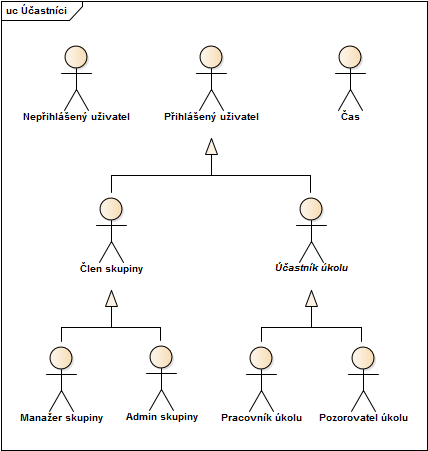
\includegraphics[width=0.7\textwidth]{ea-diagrams/uc-actors.png}
				\caption[Diagram účastníků]{Diagram účastníků aplikace}
				\label{diagram:actors}
			\end{figure}
			
			
			
		\subsection{Případy užití}
			\label{sec:usecases}
			Případy užití získané analýzou \textit{user stories} zobrazuji v diagramech případů užití. Rozdělil jsem je do čtyř balíků podle jejich účastníků pro lepší přehlednost.
			
			\subsubsection{Nepřihlášený uživatel}
			V diagramu \ref{diagram:uc-unauthorized} jsou zachyceny případy užití pro Nepřihlášeného uživatele.
			\begin{figure}\centering
				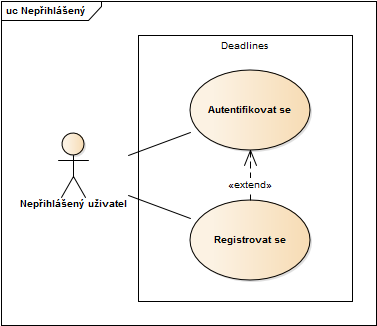
\includegraphics[width=0.6\textwidth]{ea-diagrams/uc-unauthorized.png}
				\caption[Případy užití nepřihlášených uživatelů]{Diagram případů užití pro nepřihlášeného uživatele}
				\label{diagram:uc-unauthorized}
			\end{figure}
			
			\begin{description}
				\item[UC 1.01 Registrovat se] \hfill \\
					Umožní uživateli aplikace zaregistrovat se. Zadá svoje unikátní uživatelské jméno, e-mail, heslo a jméno.
					
				\item[UC 1.02 Autentifikovat se] \hfill \\
					Umožní uživateli autentifikovat se pomocí svého uživatelského jména a hesla.	
					
			\end{description}
		
		
			\subsubsection{Případy užití pro jednotlivce}	
			V diagramu \ref{diagram:uc-logged-user} a \ref{diagram:uc-task-members} jsou zachyceny případy užití aplikace jednotlivci. V prvním diagramu jsou případy užití z pohledu Přihlášeného uživatele v druhém pak z pohledu Pozorovatele a Pracovníka úkolu.
			
			
			
			\begin{description}
				\item[UC 2.01 Upravit svůj profil] \hfill \\
					Umožní uživateli upravit si své jméno, heslo a e-mail.
				
				\item[UC 2.02 Vytvořit úkol] \hfill \\
					1. Scénář začíná, když se uživatel rozhodne vytvořit nový úkol. \\
					2. Uživatel zašle požadavek s informacemi k vytvoření úkolu, povinně název a typ. Pokud je typ \uv{S deadlinem},  pak je povinné i datum a čas deadlinu. Pokud je typ \uv{rostoucí}, pak je povinná rychlost růstu. Volitelně může zadat popis, pracnost, prioritu a seznam skupin. \\
					3. Pokud některé povinné informace chybí, scénář končí. \\
					4. Pokud uživatel není alespoň Manažerem všech skupin, které zadal, scénář končí. \\
					5. Aplikace vytvoří úkol, uživatel se stane jeho Pozorovatelem a úkol bude nasdílen všem zadaným skupinám. \\
				
				\item[UC 2.03 Sdílet úkol] \hfill \\
					1. Scénář začíná, když chce Účastník sdílet úkol. \\
					2. <Zobrazit seznam uživatelů> \\
					3. <Zobrazit seznam skupin> \\
					4. Účastník zašle požadavek obsahující úkol, uživatele a skupiny, se kterými chce úkol sdílet. \\
					5. Aplikace pošle zadaným uživatelům a skupinám nabídku ke sdílení úkolu.
				
				\item[UC 2.04 Zobrazit seznam mých úkolů] \hfill \\
					1. Scénář začíná, když chce uživatel zobrazit své úkoly.\\
				    2. <Filtrovat úkoly> \\
				    3. <Řadit úkoly> \\
				    4. Uživatel zašle požadavek na zobrazení úkolů s vybranými filtry a řazením.\\
					5. Aplikace vrátí seznam všech úkolů, kterých je uživatel součástí, se zvolenými parametry. Zobrazené informace budou identifikátor, jméno, priorita, status, urgentnost, \textit{deadline} či rychlost růstu, odpracovanost a typ. \\
					
				\item[UC 2.05 Filtrovat úkoly] \hfill \\
					Úkoly je možné filtrovat podle role uživatele v nich (pozorovatel nebo pracovník), podle jejich typu (s deadlinem nebo rostoucí), stavu a priority (pět úrovní).
					
				\item[UC 2.06 Řadit úkoly] \hfill \\
					Úkoly je možné řadit podle zvoleného kritéria. Tím může být název, datum začátku nebo \textit{deadlinu} úkolu, rozpracovanost (v procentech odpracováno ku celkové pracnosti), priorita a urgentnost.
				
				\item[UC 2.07 Rozhodnout o příchozí nabídce sdílení úkolu] \hfill \\
					1. Scénář začíná, když chce uživatel přijmout nebo zamítnout nabídku ke sdílení úkolu. \\
					2. <Zobrazit seznam příchozích nabídek na sdílení úkolu> \\
					3. Uživatel zašle požadavek s jeho rozhodnutím a nabídkou, které se týká. \\
					4. Pokud je nabídka přijata, stává se uživatel pozorovatelem sdíleného úkolu. V opačném případě je nabídka smazána. \\
				
				\item[UC 2.08 Zobrazit seznam nabídek na sdílení úkolu] \hfill \\
					Zobrazí seznam nabídek pro uživatele k připojení se ke sdílenému úkolu, v němž bude u každé nabídky uvedeno uživatelské a skutečné jméno sdílejícího uživatele a název úkolu.
				
				\item[UC 2.09 Založit pracovní skupinu] \hfill \\
					1. Scénář začíná, když chce uživatel založit pracovní skupinu. \\
					2. <Zobrazit seznam uživatelů> \\
					3. Uživatel zašle požadavek obsahující jméno skupiny a volitelně její popis. \\
					4. Aplikace vytvoří novou skupinu s daným názvem a popisem. Zakládající uživatel se stane jejím Adminem. \\
					
				\item[UC 2.10 Rozhodnout o příchozí nabídce ke vstupu do skupiny] \hfill \\
					Uživatel rozhodne, zda chce přijmout nebo odmítnout nabídku ke vstupu do skupiny. Pokud ji přijme, stane se jejím Členem.
					
				\item[UC 2.11 Zobrazit seznam nabídek ke vstupu do skupiny] \hfill \\
					Zobrazí seznam nabídek ke vstupu do skupin. U každé nabídky bude uvedeno jméno skupiny, uživatelské a skutečné jméno uživatele, od něhož nabídka pochází.
				
				\item[UC 2.12 Zobrazit seznam uživatelů] \hfill \\
					Zobrazí seznam uživatelů aplikace. U uživatele bude uvedeno jeho identifikátor, e-mail, uživatelské a skutečné jméno.
					
				\item[UC 2.13 Zobrazit seznam skupin] \hfill \\
					Zobrazí seznam skupin v aplikaci. U skupiny bude uveden její identifikátor, jméno a informace o Adminovi -- identifikátor, uživatelské i skutečné jméno a e-mail.
					
				\item[UC 2.14 Filtrovat skupiny] \hfill \\
					Umožňuje filtrovat skupiny podle toho, zda je uživatel jejich Členem a v jaké roli.
					
				\item[UC 2.15 Zobrazit úkol] \hfill \\
					1. Scénář začíná, když chce uživatel zobrazit detaily úkolu. \\
					2. <Zobrazit seznam mých úkolů> \\
					3. Uživatel zašle požadavek k zobrazení úkolu. \\
					4. Pokud uživatel není účastníkem úkolu, scénář končí.  \\
					5. Aplikace zobrazí všechny informace o úkolu, tedy identifikátor, název, popis, datum a čas začátku a \textit{deadlinu}, případně rychlost růstu. Dále pracnost, prioritu, typ, stav, urgentnost, záznamy o práci a seznam jeho Pracovníků, Pozorovatelů a zúčastněných skupin. \\
					
					
				%%%%%%%%%%%%%%%%%%%%%%%%%%%%%%%%%%%%%%%%%%%%%%%%%%%%%%%%%%%%%%%
				% Diagramy %
				%%%%%%%%%%%%
				\begin{figure}\centering
					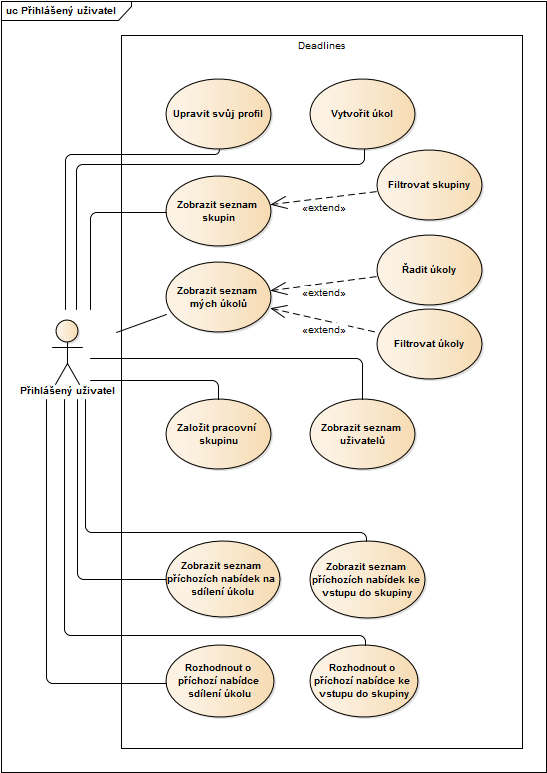
\includegraphics[width=0.9\textwidth]{ea-diagrams/uc-logged-user.png}
					\caption[Případy užití přihlášeného uživatele]{Diagram případů užití pro přihlášeného uživatele}
					\label{diagram:uc-logged-user}
				\end{figure}
				
				\begin{figure}\centering
					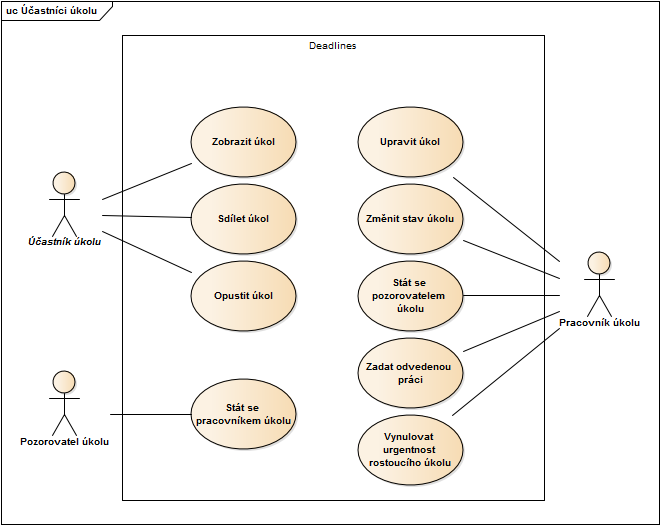
\includegraphics[width=0.7\textwidth]{ea-diagrams/uc-task-members.png}
					\caption[Případy užití účastníky úkolu]{Diagram případů užití pro účastníky úkolu}
					\label{diagram:uc-task-members}
				\end{figure}
				%%%%%%%%%%%%%%%%%%%%%%%%%%%%%%%%%%%%%%%%%%%%%%%%%%%%%%%%%%%%%%%
				
				
				\item[UC 2.16 Stát se pracovníkem úkolu] \hfill \\
					Umožňuje Pozorovateli úkolu stát se jeho Pracovníkem.				
								
				\item[UC 2.17 Změnit stav úkolu] \hfill \\
					Umožňuje Pracovníkovi změnit stav úkolu na jakýkoliv z jeho možných stavů.
				
				\item[UC 2.18 Upravit úkol] \hfill \\
					Umožňuje Pracovníkovi upravit u úkolu jeho název, popis, \textit{deadline}, pracnost a prioritu.
				
				\item[UC 2.19 Stát se pozorovatelem úkolu] \hfill \\
					Umožňuje Pracovníkovi úkolu stát se jeho Pozorovatelem.
					
				\item[UC 2.20 Zadat odvedenou práci] \hfill \\
					1. Scénář začíná, když uživatel odvedl nějakou práci a chce ji na úkolu zaznamenat. \\
					2. <Zobrazit úkol> \\
					3. Uživatel zašle požadavek s identifikátorem úkolu a počtem odpracovaných hodin. \\
					4. Pokud uživatel není Pracovníkem daného úkolu, scénář končí.
					5. Aplikace k úkolu přidá zadaný počet odpracovaných hodin. \\
					
				\item[UC 2.21 Vynulovat urgentnost rostoucího úkolu] \hfill \\
					Umožňuje Pracovníkovi vynulovat urgentnost rostoucího úkolu.
					
				\item[UC 2.22 Opustit úkol] \hfill \\
					Umožňuje Účastníkovi úkolu opustit ho. Účastníkem úkolu je možné být přímo nebo skrze skupinu. Opustit úkol lze pouze, pokud je Účastník součástí úkolu přímo.
				
					1. Scénář začíná, když se Účastník úkolu rozhodne opustit úkol. \\
					2. <Zobrazit úkol> \\
					3. Účastník zašle požadavek na opuštění úkolu. \\
					4. Pokud nebyl úkol sdílen přímo s Účastníkem (ale jen skupinou, ve které je Členem), scénář končí. \\
					5. Aplikace odebere Účastníka z úkolu. Pokud byl ale Účastník navíc součástí úkolu skrze skupinu, jíž je členem, nadále zůstane součástí úkolu skrze tuto skupinu.
			\end{description}
			
			
			
			
			\subsubsection{Případy užití pro skupiny}
			V diagramu \ref{diagram:uc-shared} jsou zachyceny případy užití aplikace členy pracovních skupin. Týkají se správy skupinových úkolů a skupin samotných. 
			
			% TODO Pokud je diagram moc velký, přesunout do přílohy?
			\begin{figure}\centering
				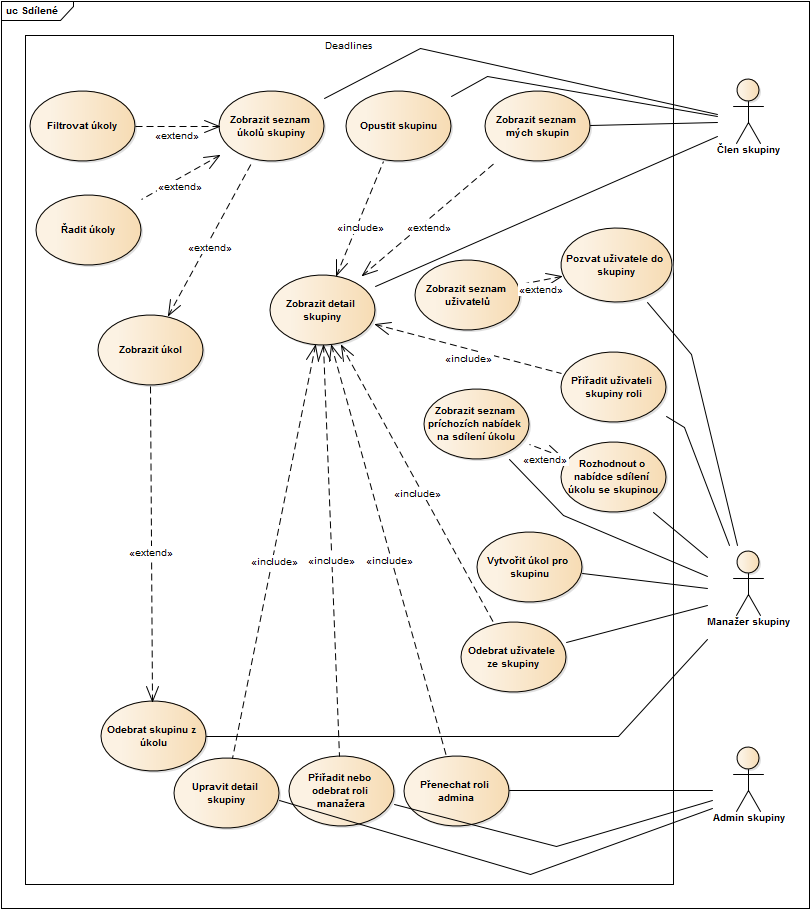
\includegraphics[width=1.0\textwidth]{ea-diagrams/uc-shared.png}
				\caption[Případy užití skupin]{Diagram případů užití pro členy pracovní skupiny}
				\label{diagram:uc-shared}
			\end{figure}
			
			% TODO projít usecases a u všech doplnit podmínky, jestli má uživatel právo to vykonat?
			\begin{description}
				\item[UC 3.01 Zobrazit seznam úkolů skupiny] \hfill \\
					1. Scénář začíná, když chce Člen skupiny zobrazit úkoly své skupiny. \\
					2. <Filtrovat úkoly> \\
					3. <Řadit úkoly> \\
					4. Uživatel zašle požadavek na zobrazení úkolů dané skupiny se zvolenými filtry a řazením. \\
					5. Pokud Člen nepatří do zvolené skupiny, je zobrazení odepřeno a scénář končí. \\
					6. Aplikace vrází seznam všech úkolů skupiny se zvolenými parametry. \\
					
				\item[UC 3.02 Opustit skupinu] \hfill \\
					1. Scénář začíná, když chce Člen opustit skupinu. \\
					2. <Zobrazit seznam mých skupin> \\
					3. Člen zašle požadavek na opuštění skupiny. \\
					4. Pokud je Člen Adminem skupiny, opuštění je zamítnuto a scénář končí. \\
					5. Aplikace odebere Člena ze skupiny a ze všech úkolů, jichž byl součástí skrze opouštěnou skupinu.
				
				\item[UC 3.03 Zobrazit seznam mých skupin] \hfill \\
					Zobrazí Členovi seznam názvů všech skupin, ve kterých je Členem.
				
				\item[UC 3.04 Zobrazit detail skupiny] \hfill \\
					1. Scénář začíná, když Člen chce zobrazit detaily skupiny. \\
					2. <Zobrazit seznam mých skupin> \\
					3. Člen zašle požadavek na zobrazení detailů dané skupiny. \\
					4. Pokud Člen nepatří do zvolené skupiny, je zobrazení odepřeno a scénář končí. \\
					5. Aplikace zobrazí detaily skupiny, tedy její jméno, popis, seznam Členů, Manažerů a Admina.
				
				\item[UC 3.05 Pozvat uživatele do skupiny] \hfill \\
					1. Scénář začíná, když Manažer chce pozvat uživatele do skupiny. \\
					2. <Zobrazit seznam uživatelů> \\
					3. Manažer pošle požadavek obsahující uživatele, které chce pozvat do skupiny. \\
					4. Aplikace vytvoří abídku ke vstupu do skupiny zadaným uživatelům. \\
				
				\item[UC 3.06 Přiřadit Členovi roli na úkolu] \hfill \\
					Umožňuje přiřadit Členům skupiny roli Pozorovatele nebo Pracovníka na úkolech skupiny.
					
				\item[UC 3.07 Zobrazit seznam nabídek na sdílení úkolu se skupinou] \hfill \\
					Zobrazí seznam příchozích nabídek ke sdílení úkolů. U nabídky bude uživatelské a skutečné jméno uživatele, od kterého pochází, a název úkolu, kterého se týká.
					
				\item[UC 3.08 Rozhodnout o nabídce sdílení úkolu se skupinou] \hfill \\
					1. Scénář začíná, když Manažer chce rozhodnout o nabídce sdílení úkolu se skupinou. \\
					2. <Zobrazit seznam nabídek na sdílení úkolu se skupinou> \\
					3. Manažer pošle požadavek na přijetí či odmítnutí nabídky. \\
					4. Aplikace provede požadovanou akci. Pokud Manažer nabídku odmítá, je smazána. Pokud Manažer nabídku přijímá, Aplikace úkol zařadí mezi úkoly skupiny a všichni Členové skupiny se stanou jeho Pozorovateli.
				
				\item[UC 3.09 Vytvořit úkol pro skupinu] \hfill \\
					1. Scénář začíná, když Manažer chce vytvořit úkol pro skupinu. \\
					2. Include(Vytvořit úkol) %TODO má to tu být, nebo smazat?
				
				\item[UC 3.10 Odebrat uživatele ze skupiny] \hfill \\
					Umožňuje Manažerovi odebrat zvoleného uživatele ze skupiny. Ten je odebrán ze všech úkolů, jichž byl součástí skrze skupinu. Pokud se jedná o Manažera nebo Admina, je odebrání zakázáno. 
				
				\item[UC 3.11 Odebrat skupinu z úkolu] \hfill \\
					1. Scénář začíná, když chce Manažer odebrat skupinu z úkolu, aby už nebyla jeho součástí. \\
					2. <Zobrazit seznam úkolů skupiny> \\
					3. Manažer zašle požadavek na odebrání skupinu z vybraného úkolu. \\
					4. Aplikace odebere úkol ze skupiny. U úkolu odebere skupinu a všechny Členy skupiny, pokud nejsou součástí úkolu i mimo skupinu. \\
					
				\item[UC 3.12 Upravit detail skupiny] \hfill \\
					Umožňuje Adminovi měnit popis skupiny.
				
				\item[UC 3.13 Přiřadit nebo odebrat roli manažera] \hfill \\
					Umožňuje Adminovi přiřazovat a odebírat roli Manažera u všech Členů skupiny.
					
				\item[UC 3.14 Přenechat roli admina] \hfill \\
					Umožňuje Adminovi přenechat svou roli jinému členovi skupiny.
					
				\item[UC 3.15 Smazat skupinu] \hfill \\
					1. Scénář začíná, když se Admin rozhodne smazat skupinu. \\
					2. <Zobrazit detail skupiny>\\
					3. Admin zašle požadavek na smazání skupiny. \\
					4. Aplikace odebere všechny ostatní členy ze skupiny -- Include(\uv{Odebrat uživatele ze skupiny}). \\
					5. Aplikace odebere skupinu ze všech jejích úkolů -- Include(\uv{Odebrat skupinu z úkolu}). \\
					6. Aplikace odebere Admina ze skupiny. \\
					7. Aplikace smaže skupinu. \\
					
			\end{description}
				
				
			
			Diagram \ref{diagram:uc-time} zachycuje časově závislé případy užití, které se pravidelně vykonávají bez přičinění uživatelů aplikace.
			\begin{figure}\centering
				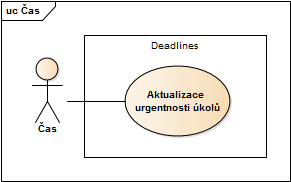
\includegraphics[width=0.5\textwidth]{ea-diagrams/uc-time.png}
				\caption[Případy užití časových událostí]{Diagram případů užití pro časově závislé události}
				\label{diagram:uc-time}
			\end{figure}
			
			\begin{description}
				\item[UC 4.01 Zvýšení urgentnosti úkolů] \hfill \\
					1. Scénář začíná po uplynutí časového intervalu pro zvyšování urgentnosti úkolů. \\
					2. Aplikace načte všechny úkoly, jejichž stav není Splněný ani Zrušený a které nebyly aktualizovány v nedávné době. Určení \uv{nedávné doby} je možné v nastavení aplikace. \\
					4. Aplikace vypočte novou hodnotu urgentnosti pro každý z úkolů. \\
			\end{description}
			
			
			
			
			
		
		

		
	\section{Doménový model}
		\label{sec:domain-model}
		Doménový model slouží k popisu dat, zachycení hlavních entit, se kterými bude aplikace pracovat, a vztahů mezi nimi. \cite{domain-model} Jedná se o abstraktní pohled na problém, a tak diagram obsahuje jen entity a jejich vlastnosti dané předchozími kroky analýzy. Nejsou v něm implementační detaily, jako například konkrétní atributy a metody.
		
		Diagram doménového modelu je znázorněn na obrázku \ref{diagram:domain-model}. Znázorňuje vztahy mezi entitami a některá omezení, jako například vzájemnou výlučnost. \cite{domain-model-multiple-association} V této části se dále budu věnovat popisu jednotlivých entit modelu.
		
		\subsection{User}
			Entita User reprezentuje uživatele aplikace. Uchovává jeho uživatelské jméno, které je unikátní v rámci aplikace, e-mail, jméno a heslo k jeho přihlášení.
			
		\subsection{Group}
			Entita Group reprezentuje pracovní skupinu. Má název a popis. Uživatelé s ní mohou být ve třech různých vztazích -- jako Člen, Manažer, nebo Admin. 
		
		\subsection{Task}
			Entita Task reprezentuje úkol. Obsahuje informace stanovené v předchozích krocích analýzy. Uživatel může být součástí úkolu jako pozorovatel, nebo pracovník. Nemůže být ale oboje zároveň. 
		
		\subsection{DeadlineTask}
			Entita DeadlineTask je typ entity Task, reprezentující úkol s \textit{deadlinem}. 
		
		\subsection{GrowingTask}
			Entita GrowingTask je typ entity Task, reprezentující rostoucí úkol. Obsahuje informaci o rychlosti růstu.
		
		\subsection{TaskParticipant}
			TaskParticipant je entita reprezentující dvojici entit User--Task. Tato dvojice je v aplikaci unikátní, takže nemohou existovat dvě stejné zároveň. 
			
			Skrze tuto entitu je uživatel součástí úkolu. Součástí úkolu může být sám, pokud je nastaven příznak \texttt{solo}, nebo jako člen skupiny či skupin, pokud jsou k entitě TaskParticipant přiřazeny.
		
		\subsection{TaskWork}
			Entita TaskWork reprezentuje práci vykonanou na úkolu uživatelem. Je spjata s entitami User a Task, takže i když uživatel úkol opustí a odpovídající TaskParticipant zanikne, pořád bude záznam o jeho práci na úkolu existovat.
		
		\subsection{Offer}
			Entita Offer reprezentuje nabídku, kterou uživatel někomu zasílá.
		
		\subsection{TaskSharingOffer}
			Entita TaskSharingOffer je typ nabídky, která reprezentuje nabídku ke sdílení úkolu.
		
		\subsection{UserTaskSharingOffer}
			Entita UserTaskSharingOffer je typ nabídky ke sdílení úkolu, která je určena pro uživatele. Vznikne, pokud jeden uživatel chce k úkolu, na kterém pracuje, pozvat jiného uživatele.
		
		\subsection{GroupTaskSharingOffer}
			Entita UserTaskSharingOffer je typ nabídky ke sdílení úkolu, která je určena pro skupinu. Vznikne, pokud jeden uživatel chce k úkolu, na kterém pracuje, pozvat skupinu.
		
		\subsection{MembershipOffer}
			Entita MembershipOffer je typ nabídky, která reprezentuje nabídku ke vstupu do skupiny. Vznikne, pokud manažer skupiny do ní chce pozvat nového uživatele.
		
	
%%%%%%%%%%%%%%%%%%%%%%%%%%%%%%%%%%%%%%%%%%%%%%%%%%%%%%%%%%%%%%%%%%%%%%%%%%%%%%%%%%%%%%%%%%%%%%%%%%%%%%%%%
%%%%%%%%%%%%%%%%%%%%%%%%%%%%%%%%%%%%%%%%%%%%%%%%%%%%%%%%%%%%%%%%%%%%%%%%%%%%%%%%%%%%%%%%%%%%%%%%%%%%%%%%%

\chapter{Návrh řešení}
	\label{chapter:design}
	
	V této kapitole představím technologie zvolené k vypracování aplikace a navrhnu REST API, které bude aplikace nabízet. Dále se budu věnovat architektuře aplikace, návrhovému modelu tříd a databázovému modelu. Tím vytvořím podklad pro následující implementaci prototypu aplikace pomocí zvolených technologií.

	\section{Technologie}
	
		\subsection{Java}
			Již v zadání práce je avizováno, že aplikace bude postavena na platformě Java. \cite{java} Jazyk Java byl vyvinutý společností Sun Microsystems a veřejnosti představen v roce 1996. Syntaxí je podobný C/C++ a je silně objektově orientovaný. Program napsaný v Javě je kompilován do podoby \textit{bytecode}, který je následně spouštěn na \textit{Java Virtual Machine} (JVM), který bytecode interpretuje. To znamená, že jazyk je platformně nezávislý -- \textit{bytecode} vzniklý kompilací zdrojového Java kódu je možné spustit na jakékoliv platformě, pokud na ní je přítomný odpovídající \textit{JVM}. 
			
			Oproti jazykům C/C++ navíc Java disponuje automatickou správou paměti, nazvanou \textit{garbage collection}, takže vývojáři se nemusí tolik starat o životní cyklus objektů a následné \textit{memory leaks}. \cite{what-is-java} \cite{pjv-java}
		
		\subsection{Spring}
			Spring je framework, který zjednodušuje tvorbu enterprise aplikací v Javě. \cite{spring} Jednou z výhod Springu je jeho podpora návrhového vzoru \textit{dependency injection}, díky kterému je program lépe modularizovatelný, testovatelný a znovupoužitelný.\cite{dependency-injection}
			
			Další součástí Springu je webový modul \textit{Web MVC framework}. \cite{spring-mvc-framework} Ten umožňuje tvorbu webových aplikací podle architektonického vzoru MVC. Je také možné využít ho pro tvorbu \textit{RESTful} aplikace, což je cílem implementační části této práce.
			
			\subsubsection{Spring Boot}
				Nadstavbou k frameworku Spring je projekt Spring Boot. \cite{spring-boot} Vztah mezi Spring a Spring Boot je zobrazen na obrázku \ref{pic:spring-boot}. Byl vyvinut k usnadnění tvorby Spring aplikací. Představuje více \uv{dogmatický} (\textit{opinionated}) pohled na Spring, což znamená, že od vývojáře očekává \uv{standardní} chování podle zaběhlých postupů. \cite{opinionated-software} Vývojáře za to ale odstiňuje od nutnosti (nejen) počáteční konfigurace a nabízí navíc některé funkce, jako \textit{embedded server}, bezpečnost, metriky, kontrolu stavu aplikace a další. V případě, že výchozí konfigurace nevyhovuje, je možné si ji ručně přizpůsobit. \cite{spring-boot-blog}
				
				Spring Boot také umožňuje sestavit aplikaci do podoby jednoho JAR souboru (\uv{\textit{fat jar}}), který obsahuje vše, co je nutné k jejímu spuštění. Není tedy potřeba mít pro nasazení zprovozněný aplikační server, jako například Tomcat či GlassFish. Stále je ale možné aplikaci sestavit do WAR souboru a vlastní server použít.
				
				\begin{figure}\centering
					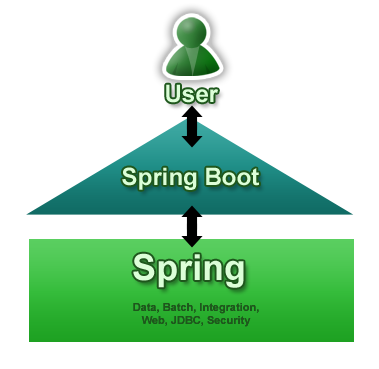
\includegraphics[width=0.5\textwidth]{spring-boot.png}
					\caption[Spring Boot]{Vztah Spring a Spring Boot \cite{spring-boot-blog}}
					\label{pic:spring-boot}
				\end{figure}
				
		\subsection{Hibernate}
			Hibernate \cite{hibernate} je framework pro platformu Java, usnadňující persistenci dat. Jedná se o nástroj pro ORM (objektově-relační mapování), který se stará o transformaci objektů aplikace do podoby vhodné pro uložení do relační databáze, jejich uložení, a následné načtení a transformaci z databáze zpět na objekty. Způsob mapování objektů do databáze lze nastavit buď v konfiguračním XML souboru, nebo přímo ve zdrojovém kódu anotacemi.
			
			Kromě usnadnění práce s databází je další výhodou Hibernate možnost jednoduché změny uložiště. Kód aplikace komunikuje s jeho API stejným způsobem, nehledě na typ databáze, ke které je připojen.
		
		\subsection{MySQL}
			Persistence dat aplikace bude zprostředkována relační databází. Pro výběr databáze jsem se řídil jejich popularitou a podmínkou použití zdarma. Nejpopulárnější takovou databází je MySQL. \cite{db-ranking} Aplikace nebude mít takové požadavky na persistentní vrstvu, aby nějak ovlivnily výběr databáze. Funkce, které budou potřeba, splňují všechny uvažované možnosti. Větší popularita MySQL bude znamenat lepší podporu komunity a snažší řešení problémů během implementace.
			
		\subsection{Apache Tomcat}
			Pro nasazení aplikace bude použit server Apache Tomcat. \cite{tomcat} Je nenáročný na hardware a jednoduchý na zprovoznění. 
		
	
	\section{REST API}
		V této sekci nejprve krátce vysvětlím pojmy API a REST API. Poté přistoupím k návrhu konkrétního REST API pro aplikaci Deadlines.
	
		\subsection{API}
			API (\textit{Application Programming Interface}) slouží k jednoduché a spolehlivé komunikaci mezi aplikacemi nebo moduly aplikace. API představuje kontrakt, kterým se \textit{producent} zavazuje k nabízení svých služeb v dané zdokumentované podobě, jež mohou být využity \textit{konzumenty}.
			
			Autoři knihy \textit{APIs: A Strategy Guide} \cite{apis-a-strategy-guide} definují API takto: (Přeloženo mnou z anglického originálu.)
			
			\textit{API je v podstatě kontrakt. Ve chvíli, kdy tento kontrakt existuje, vývojáři tíhnou k využívání API, protože ví, že se na něj mohou spolehnout. Kontrakt zvyšuje důvěru, což zlepšuje použitelnost. Tento kontrakt také zefektivňuje spojení mezi producentem a konzumentem, protože rozhraní jsou dokumentována, jsou konzistentní a předvídatelná.} 
	
		\subsection{REST}
			Termín REST (REpresentational State Transfer) byl poprvé zaveden v roce 2000 Royem Fieldingem v jeho dizertační práci. \cite{rest-dissertation} Ve zkratce se jedná o koncept designu distribuované architektury. Definuje rozhraní, které je použitelné pro jednotný přístup ke zdrojům (resources). Těmi mohou být data nebo stavy aplikace, popsatelné konkrétními daty.
			Zdroje v kontextu REST jsou identifikované pomocí URI a komunikovány mezi klientem a serverem v podobě reprezentací v libovolné textové, strojově zpracovatelné podobě (například JSON nebo XML). \cite{rest-youtube}
			
			Architektonický styl REST popisuje šest podmínek:
			\begin{itemize}
				\item uniform interface (jednotné rozhraní), 
				\item stateless (bezstavovost),
				\item cacheable (cachovatelnost),
				\item client-server,
				\item layered system (systém z vrstev),
				\item code on demand (kód na vyžádání).
			\end{itemize}
			Popis architektury REST není předmětem této práce, takže se mu dále nebudu věnovat.
			
		\subsection{REST API aplikace Deadlines}
			%API aplikace budu dokumentovat ve formátu API Blueprint. \cite{api-blueprint} Ten představuje jednoduchý způsob, jak popsat zdroje, jejich \textit{endpointy}, návratové hodnoty a další informace. Jeho syntaxe vychází z jazyka Markdown. \cite{markdown} 
			
			
			%TODO příloha, nebo online?
			Kompletní popis API, včetně požadovaného obsahu požadavků a možných odpovědí, je vypsán v příloze v sekci \ref{appdx:restapi} a dostupný na webu Apiary\cite{apiary-api}. Zde uvedu možné odpovědi aplikace na požadavky, dostupné \textit{endpoints} a popíšu jejich funkci. 
			
			Pokud není uvedeno jinak, všechna volání API musí být autentifikovaná použitím \textit{HTTP Basic Access Authentication}. \cite{http-basic-auth} Jméno a heslo pro \textit{Basic Authentication} jsou uživatelské jméno a heslo uživatele.
			
			Těla požadavků i odpovědí jsou ve formátu JSON, obsah hlavičky \textit{Content-Type} je \textit{application/json}.
			
			\subsubsection{Odpovědi}
			\label{sec:responses}
			Každý \textit{endpoint} odpovídá na požadavek odpovědí, která obsahuje standardní HTTP kód popisující, jak volání dopadlo, a případně tělo. Zde jsou některé z HTTP kódů:
			\begin{description}
				\item[200 OK] Požadavek proběhl v pořádku.
				\item[201 CREATED] Požadovaný objekt či záznam byl vytvořen. V hlavičce odpovědi s názvem \textit{Location} je uvedena relativní cesta k nově vytvořenému zdroji.
				\item[400 BAD REQUEST] V požadavku je chyba. Detaily o konkrétní chybě jsou obsaženy v těle zprávy.
				\item[401 UNAUTHORIZED] Požadavek neobsahuje autentifikační údaje, nebo jsou údaje chybné.
				\item[403 FORBIDDEN] Volající uživatel nemá dostatečná práva k provedení požadavku.
				\item[404 NOT FOUND] Požadovaný zdroj nebyl nalezen.
				\item[409 CONFLICT] Objekt či záznam nemohl být vytvořen, protože již existuje.
			\end{description}
			Chybové odpovědi mohou obsahovat v těle odpovědi další informace o chybě. Tělo má následující formát:
				\begin{Verbatim}[obeytabs,tabsize=2]
{
	"errorCode": 0,
	"errorMessage": "Sample error message."
}
				\end{Verbatim}
				Výčet možných chybových kódů se nachází v příloze v sekci \ref{appdx:rest-error-codes}.
			
			\hfill \\
			
			
			\subsubsection{Endpointy}
			\label{sec:rest-api}
			\begin{description}			
			\item[\texttt{/user [GET, POST]}] \hfill \\
				GET vrátí seznam všech uživatelů v systému. \\
				POST vytvoří nového uživatele z poskytnutých dat. \\
				
				Tento \textit{endpoint} je přístupný i neautentifikovaným voláním.
				
			\item[\texttt{/user/\{user\_id\} [GET, PUT]}] \hfill \\
				GET vrátí informace uživatele s ID \texttt{user\_id}. \\
				PUT upraví profil uživatele s ID \texttt{user\_id} předanými daty. Povoleno je měnit pouze profil volajícího uživatele.
			
			\item[\texttt{/task[\{?filter\&order\}] [GET, POST]}] \hfill \\
				GET vrátí seznam všech úkolů volajícího uživatele, které odpovídají zadaným parametrům. Detailní popis možných parametrů je dostupný v příloze v sekci \ref{appdx:restapi}. \\
				POST vytvoří nový úkol z poskytnutých dat. Volající uživatel se stane jeno Pozorovatelem.
			
			\item[\texttt{/task/\{task\_id\} [GET, PUT]}] \hfill \\
				GET vrátí detailní informace o úkolu se zadaným ID. \forworkers \\
				PUT upraví úkol se zadaným ID podle informací v těle požadavku. \forworkers
			
			\item[\texttt{/task/\{task\_id\}/reseturgency [POST]}] \hfill \\
				Vynuluje urgentnost zadaného úkolu. Použitelné jen pro rostoucí úkoly. \forworkers
			
			\item[\texttt{/task/share/\{task\_id\} [POST]}] \hfill \\
				Zašle nabídku na sdílení úkolu uživatelům a skupinám předaným v těle požadavku. \forworkers
			
			\item[\texttt{/task/leave/\{task\_id\} [POST]}] \hfill \\
				Odebere volajícího uživatele z úkolu se zadaným ID. 
			
			\item[\texttt{/task/role/\{task\_id\}\{?newRole[\&targetUser\&targetGroup]\} [POST]}] \hfill \\
				Nastaví roli volajícího uživatele v úkolu se zadaným ID na roli předanou v parametru \texttt{newRole}. Pozorovatel se tak může stát Pracovníkem a naopak. 
				
				Volitelně lze také zadat ID skupiny a uživatele, jehož se má volání týkat. Pokud je volající uživatel Manažerem zadané skupiny a cílový uživatel jejím členem, pak je Manažerovi umožněno změnit roli uživatele.
			
			\item[\texttt{/task/report/\{task\_id\} [POST]}] \hfill \\
				Vytvoří záznam o odvedené práci od volajícího uživatele na úkolu s předaným ID. Detaily záznamu jsou obsaženy v těle požadavku. \forworkers
				
			\item[\texttt{/offer/task/user [GET]}] \hfill \\
				Vrátí seznam nabídek ke sdílení úkolu pro volajícího uživatele.
			
			\item[\texttt{/offer/task/user/resolve/\{task\_offer\_id\} [POST]}] \hfill \\
				Přijme nebo zamítne nabídku ke sdílení úkolu se zadaným ID. Volající uživatel musí být příjemcem nabídky.
				
			\item[\texttt{/offer/task/group/\{group\_id\} [GET]}] \hfill \\
				Vrátí seznam nabídek ke sdílení úkolu pro skupinu se zadaným ID. \formanagers
			
			\item[\texttt{/offer/task/group/\{group\_id\}/resolve/\{task\_offer\_id\} [POST]}] \hfill \\
				Přijme nebo zamítne nabídku ke sdílení úkolu se skupinou se zadaným ID. \formanagers
			
			\item[\texttt{/offer/membership [GET]}] \hfill \\
				Vrátí seznam nabídek ke vstupu do skupiny pro volajícího uživatele.
			
			\item[\texttt{/offer/membership/resolve/\{membership\_offer\_id\} [POST]}] \hfill \\
				Přijme nebo zamítne nabídku ke vstupu do skupiny s předaným ID.  Volající uživatel musí být příjemcem nabídky.
			
			\item[\texttt{/group\{?role\} [GET, POST]}] \hfill \\
				GET vrátí seznam skupin v aplikaci. Volitelný parametr \texttt{role} určuje, zda vracet všechny skupiny, nebo jen ty, jichž je volající členem v zadané roli. \\
				POST vytvoří novou skupinu z informací předaných v těle požadavku. Volající uživatel se stane jejím Adminem.
			
			\item[\texttt{/group/\{group\_id\} [GET, PUT, DELETE]}] \hfill \\
				GET vrátí detaily skupiny se zadaným ID. \formembers \\
				PUT upraví detaily skupiny se zadaným ID daty předanými v těle požadavku. \foradmin \\
				DELETE smaže skupinu se zadaným ID. \foradmin 

			\item[\texttt{/group/\{group\_id\}/member/offer [POST]}] \hfill \\
				Zašle nabídku ke vstupu do skupiny se zadaným ID uživatelům předaným v těle požadavku. \formanagers

			\item[\texttt{/group/\{group\_id\}/member/\{member\_id\} [PUT, DELETE]}] \hfill \\
				PUT upraví záznam o členovi skupiny. Změní jeho roli ve skupině na tu předanou v těle požadavku. \formanagers \\
				DELETE Odebere uživatele s ID \texttt{user\_id} ze skupiny s ID \texttt{group\_id}. \formanagers
			
			\item[\texttt{/group/\{group\_id\}/task/\{task\_id\} [DELETE]}] \hfill \\
				Odebere skupinu s ID \texttt{group\_id} z úkolu s ID \texttt{task\_id}. \formanagers
		

			\end{description}
			
			
	\section{Urgentnost}
		Jedním z funkčních požadavků je výpočet \textit{urgentnosti} úkolů. Ta má vyjadřovat důležitost úkolu v daném momentě a má pomoct uživateli rozhodnout se, na kterém úkolu bude pracovat. Čím vyšší hodnota, tím je nutnější se danému úkolu věnovat. Výpočet hodnoty urgentnosti bude záviset na typu úkolu. Způsob výpočtu pro oba typy úkolů popíšu ve zbytku této sekce.
		
		Hodnota urgentnosti bude reálné číslo v intervalu $\langle 0; 200 \rangle$. Hodnota 100 značí, že by měl uživatel na úkolu začít pracovat v tuto chvíli. Např. pro úkol s deadlinem urgentnost 100 znamená, že do deadlinu v tuto chvíli zbývá stejně času, jako je odhad zbývající pracnosti úkolu.
	
		\subsection{Rostoucí úkol}
			Rostoucí úkol obsahuje informaci o rychlosti růstu urgentnosti. Tato hodnota představuje, za kolik hodin má být urgentnost rovna 100. Růst urgentnosti je lineární a řídí se vztahem
			$$
				u = \frac{1}{hrs} \cdot z \cdot 100
			$$
			kde $u$ je hodnota urgentnosti, $h$ je rychlost růstu a $z$ je počet hodin, které uběhly od vytvoření či vynulování úkolu.
		
		
		\subsection{Úkol s deadlinem}
			Úkol s deadlinem dosáhne urgentnosti 100, pokud do deadlinu zbývá přesně tolik času, jako je odhadovaná pracnost úkolu.
		
			Pro úkol s deadlinem definuji rezervu $r$ následujícím způsobem:
			\begin{equation}
				r = \frac{t}{w} + \frac{t}{d}
			\end{equation}
			kde $t$ je čas do deadlinu v hodinách, $w$ je zbývající pracnost v hodinách a $d$ je konstanta. Experimentálně jsem stanovil, že $d=5$. 
			
			První zlomek udává, v jakém poměru je zbývající čas ku pracnosti. Například pokud do deadlinu zbývá 8 hodin a zbývající pracnost je 2 hodiny, výsledkem bude 4. Druhý zlomek slouží k úpravě rezervy v závislosti na zbývajícím čase. Čím méně času zbývá, tím menší bude tento člen. To z důvodu, aby rezerva u úkolu, kterému zbývá více času, byla větší, než u úkolu, který má času méně, i když jsou poměry času ku práci stejné. 
			K této úpravě jsem přistoupil, protože chci, aby úkoly blíže deadlinu měly větší urgentnost než stejně rozpracované úkoly dále od deadlinu.
			
			Chci, aby hodnota urgentnosti rostla nejrychleji s rezervou pohybující se kolem čísla 1; urgentnost úkolů s velkou kladnou nebo zápornou rezervou není tak důležitá, jako urgentnost těch úkolů, na kterých by uživatel měl začít pracovat v tuto chvíli -- ty mají rezervu blízko číslu 1. 
			
			Urgentnost úkolu s deadlinem se tak řídí následující funkcí:
				\begin{equation}
				f(r)=
				\begin{cases}
					\lvert(a^{-r+1}-1)\cdot b \rvert +b+c& \text{pro } r\leq 0 \\
					a^{r-1}\cdot b + c& \text{pro } r\geq 0
				\end{cases}
				\end{equation}
			kde $a$, $b$ a $c$ jsou konstanty, zvolené jako $a=1.1$, $b=100$, $c=0$.

			Urgentnost úkolu nezávisí na jeho prioritě. Vzorec pro urgentnost lze ale jednoduše upravit tak, aby se priorita zohlednila, a to dosazením odpovídající hodnoty za $c$.
			
			Graf hodnoty urgentnosti vzhledem k rezervě je zobrazen na obrázku \ref{urgency-plot}.
			
			\begin{figure}\centering
				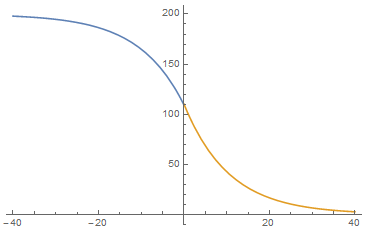
\includegraphics[width=0.7\textwidth]{resources/urgency-plot.png}
				\caption[Urgentnost úkolu s deadlinem]{Funkce urgentnosti pro úkol s deadlinem}
				\label{urgency-plot}
			\end{figure}
			


	
	\section{Autentifikace}
		Ukládání hesel uživatelů v databázi v čistém textu představuje bezpečnostní riziko. V případě, že dojde k úniku dat databáze, může útočník získat přihlašovací jména i hesla a tím i možnost přihlásit se do aplikace jako kterýkoliv uživatel. Z tohoto důvodu je vhodné neukládat samotná hesla, ale jen jejich \uv{otisk}. Ten se z hesla vytvoří pomocí \textit{hash funkce}. \cite{hash-function} Při použití vhodné funkce se jedná o relativně bezpečný způsob, kterým ověřovat uživatele, aniž by mohlo dojít k úniku jejich hesel.
		
		Nevýhodou této metody autentifikace je fakt, že pro uživatele se stejným heslem funkce vygeneruje vždy stejný otisk. To znamená, že při prolomení hesla jednoho uživatele mohou být ohroženi i další uživatelé, kteří mají stejné heslo. Navíc existují tabulky, které obsahují předpočítané výstupy hash funkcí a vstupní řetězce, které těmto výstupům odpovídají, tzv. \textit{rainbow tables}. \cite{rainbow-table} Ty mohou být použity pro zrychlení prolamování slabších hesel. 
		
		Z tohoto důvodu v aplikaci kromě hashování používám metodu \textit{solení}. Ta spočívá v tom, že se otisk negeneruje jen z hesla, ale navíc se k němu přidá náhodně vygenerovaný řetězec, tzv. \textit{sůl}. Stejná hesla tak budou mít rozdílné otisky a znemožní se využití \textit{rainbow tables} a slovníkových útoků. V databázi bude pro autentifikaci uložena dvojice \texttt{(hash(heslo, sůl), sůl)}. \cite{hash-function}
				
	\section{Architektura}
		Architektura aplikace popisuje způsob, jakým je členěna na logické celky a jak ty mezi sebou komunikují. Úroveň složitosti architektury souvisí s nefunkčními požadavky na aplikaci. Větší nároky, například na škálovatelnost, výkon, bezpečnost a další aspekty, znamenají nutnost navrhnout dostatečně robustní architekturu, která jim bude vyhovovat. 
		
		V této sekci popíšu, jak bude vypadat architektura aplikace Deadlines.
		
	\subsection{Architektura Deadlines}	
		Aplikaci navrhuji podle vzoru vícevrstvé architektury. Tvoří ji několik vrstev, z nichž každá je zodpovědná za jinou funkcionalitu. Způsob komunikace je definován rozhraním, které vrstvy nabízí. Je tak snazší oddělit konkrétní implementaci vrstev od jejich okolí. Jednou z výhod této architektury je možnost znovupoužitelnosti vrstev. To je užitečné například v případě, kde existuje několik různých rozhraní pro interakci s uživatelem. Všechny mohou komunikovat s odpovídající vrstvou, pro kterou nehraje roli jejich typy a počet.
		
		Další výhodou je možnost poměrně pohodlně měnit konkrétní implementaci dané vrstvy (zejména v kombinaci s použitím \textit{IoC}) a to bez zásahů do vrstev, které s ní komunikují. 
		
		Diagram architektury aplikace je zobrazen v příloze, na obrázku \ref{diagram:component-model}. 
		
		%TODO - chci popisovat komponenty? 
		%\subsubsection{Controllers}
		%\subsubsection{Bakground Jobs}
		%\subsubsection{Security}
		%\subsubsection{Business Services}
		%\subsubsection{Model}
		%\subsubsection{Data Access}
		%\subsubsection{Hibernate}
		%\subsubsection{Relational Database}				
	
	
	
	
	
	\section{Návrhový model}
		V této sekci se budu věnovat návrhovému modelu tříd a jeho popisu. Ten vychází z analytického modelu, rozšiřuje množství tříd a doplňuje implementační detaily. Mezi ně patří atributy a jejich typy, metody, viditelnost. Definují se zde také rozhraní, typy tříd a aplikují návrhové vzory. \cite{navrhovy-model}
		
		Ve zbytku této sekce budu popisovat jednotlivé části návrhového modelu. Obrázek zobrazující všechny třídy, rozdělené do balíčků (\textit{packages}), je k dispozici v příloze, diagram \ref{diagram:packages-root}.
		
		\subsection{Balíček \texttt{config}}
			Tento balíček obsahuje třídy využívané napříč celou aplikací. Jsou zde definovány hodnoty chybových kódů a zpráv, \textit{Beans} pro využití frameworkem Spring a nastavení pravidel pro autentifikaci na \textit{endpointech} aplikace.
			
		\subsection{Balíček \texttt{controllers}}
			Tento balíček reprezentuje vrstvu \textit{Controllers} v architektuře aplikace. Třídy \texttt{Controller} jsou zodpovědné za zpracování příchozích požadavků a zasílání odpovědí. Ověří autentifikaci požadavku a poté ho v odpovídajícím formátu delegují na vrstvu \textit{Business Service}. Odpoveď této vrstvy v odpovídajícím tvaru pošlou zpět.
			
			Třída \texttt{JsonViews} definuje hierarchii rozhraní, kterými lze filtrovat množství informací, které controller posílá v odpovědi.
			
			Balíček \texttt{httpbodies} obsahuje definice \textit{POJO} objektů, které reprezentují strukturu těl požadavků a odpovědí.
			
		\subsection{Balíček \texttt{exceptions}}
			Zde se nacházejí třídy vyjímek aplikace.
			
		\subsection{Balíček \texttt{dao}}
			Balíček reprezentuje vrstvu \textit{Data Access}, obsahuje třídy zprostředkovávající persistenci dat.
			
			Každá entita modelu zde má odpovídající podbalíček, který obsahuje rozhraní a třídy využité při jejím ukládání a načítání. Jeden z těchto podbalíčků, \texttt{group}, je zobrazen na obrázku \ref{diagram:package-dao}. Rozhraní \texttt{GroupDAO} definuje metody, které jsou nabízeny ostatním komponentám aplikace pro ukládání a načítání objektů \texttt{Group} z databáze. Třída \texttt{GroupDAOHibernate} je konkrétní implementací tohoto rozhraní, které využívá \textit{Hibernate}. Rozhraní \texttt{GroupRepository} představuje způsob komunikace právě s frameworkem \textit{Hibernate}.
			
			Balíček \texttt{processing} obsahuje třídy a rozhraní, které umožňují filtrování a řazení načítaných dat.
			
			\begin{figure}\centering
				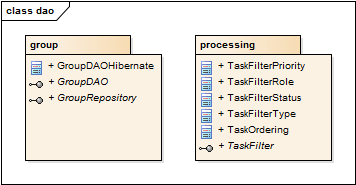
\includegraphics[width=0.7\textwidth]{ea-diagrams/packages/dao.png}
				\caption[Balíček dao]{Detail tříd balíčku dao}
				\label{diagram:package-dao}
			\end{figure}
				
		\subsection{Balíček \texttt{services}}
			Detailní pohled na balíček je na obrázku \ref{diagram:package-services}. 
			
			Služby v balíčku reprezentují vrstvu \textit{Business Services}. Balíček obsahuje rozhraní definující operace, které je možné v aplikaci provádět, a v podbalíčku \texttt{implementation} třídy, které ho implementují.
			
			Podbalíček \texttt{security} obsahuje interní služby pro autentifikování příchozích požadavků a pro kontrolu, zda mají volající uživatelé dostatečná práva k provádění požadovaných akcí.
			
			Podbalíček \texttt{helpers} obsahuje interní služby pro práci s entitami, které jsou využívány službami, ale nejsou součástí API této vrstvy.
			
			\begin{figure}\centering
				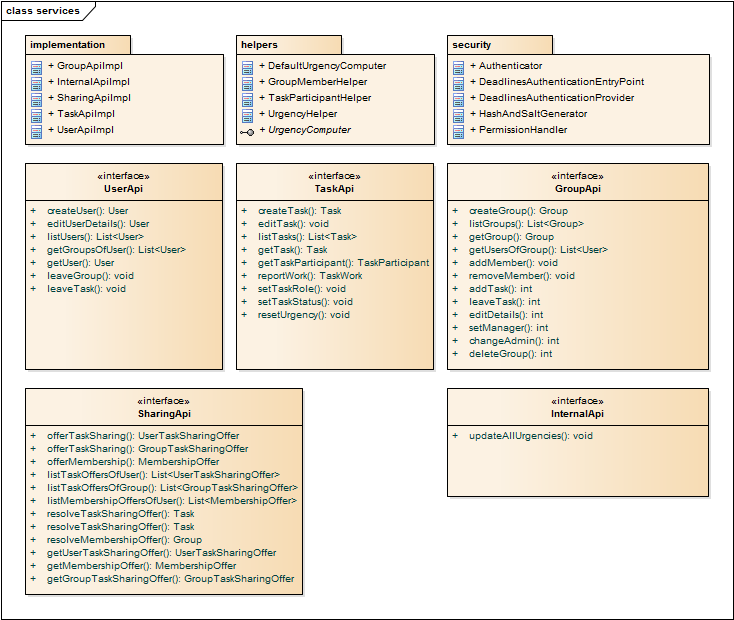
\includegraphics[width=1\textwidth]{ea-diagrams/packages/services.png}
				\caption[Balíček services]{Detail tříd balíčku services}
				\label{diagram:package-services}
			\end{figure}
			
		\subsection{Balíček \texttt{jobs}}
			Balíček reprezentuje v architektuře vrstvu \textit{Background Jobs}. Třídy v něm spouští periodické akce, které se mají v systému vykonávat. Příkladem takové akce je pravidelné přepočítání urgentnosti všech aktivních úkolů.
			
		\subsection{Balíček \texttt{utils}}
			Zde jsou zařazeny pomocné třídy, které nabízí různé statické metody, využívané zejména při testování.
			
		\subsection{Balíček \texttt{model}}
			Tento balíček odpovídá stejnojmenné komponentě z diagramu architektury. Obsahuje třídy, které reprezentují business entity aplikace, analyzované v sekci \ref{sec:domain-model}. Třídy v sobě drží informace prostřednictvím atributů a relací k dalším třídám tohoto balíčku. Mají jen základní metody pro čtení a ukládání atributů. Veškerá manipulace se vztahy mezi třídami a udržování konzistentních referencí v případě obousměrných vztahů je zodpovědností \textit{Business Services} vrstvy. 
			
			Diagram popisující detaily tříd a vztahy mezi nimi je zobrazen v příloze, na obrázku \ref{diagram:class-model}.
			
		\subsection{Třída \texttt{DeadlinesApplication}}
			Metoda \texttt{main()} této třídy je vstupním bodem celé aplikace.
		
		
	
	\section{Databázový model}
		Databázový model popisuje způsob uložení dat do databáze. Udává, jaké tabulky a sloupce v databázi existují, jaké mají klíče a integritní omezení. Dekomponují se v něm vztahy kardinality \textit{m:n} vytvořením pomocné tabulky.
		
		Databázový model vznikl na základě doménového a návrhového modelu a je zobrazen v příloze na obrázcích \ref{diagram:database-model-base} a \ref{diagram:database-model-offers}. Diagram byl z důvodu přehlednosti rozdělen na dvě části. První diagram zobrazuje tabulky databáze kromě nabídek, druhý zobrazuje tabulky nabídek a jejich vztah k tabulkám v prvním diagramu.
		
		V návrhovém modelu je několik tříd, které tvoří dědičnou hierarchii a tu je potřeba převést do reprezentace tabulkami. Na to existuje několik postupů:
		\begin{itemize}
			\item Jedna tabulka pro rodiče, která obsahuje sjednocení atributů všech jejích potomků a sloupec identifikující typ záznamu.
			\item Tabulka pro každou konkrétní třídu.
			\item Tabulka pro rodiče a s ní asociovaná tabulka pro každého z potomků, obsahující atributy v něm definované.
		\end{itemize}
		
		Pro uložení dědičné hierarchie třídy \texttt{Task} jsem zvolil první způsob. Rozdíl mezi podtypy této třídy je jen v jediném atributu, takže při ukládání záznamů bude množství nevyužitých sloupců minimální.
		
		Pro uložení třídy \texttt{Offer} jsem zvolil druhý způsob. Všechny podtypy mají společný atribut identifikující uživatele, který jej vytvořil, ale v ostatních atributech se liší. Proto má každý podtyp svou vlastní tabulku.
		
		Inicializační SQL skript pro vytvoření databáze je přiložen na médiu. %TODO kde je SQL skript?
	
	


%%%%%%%%%%%%%%%%%%%%%%%%%%%%%%%%%%%%%%%%%%%%%%%%%%%%%%%%%%%%%%%%%%%%%%%%%%%%%%%%%%%%%%%%%%%%%%%%%%%%%%%%%
%%%%%%%%%%%%%%%%%%%%%%%%%%%%%%%%%%%%%%%%%%%%%%%%%%%%%%%%%%%%%%%%%%%%%%%%%%%%%%%%%%%%%%%%%%%%%%%%%%%%%%%%%

\chapter{Implementace}
	\label{chapter:implementation}
	
	V této kapitole se budu věnovat bližšímu popisu průběhu implementace aplikace. % TODO
	
	\section{Vývojové prostředí}
		Aplikaci jsem vyvíjel v prostředí IntelliJ IDEA od firmy JetBrains. Poskytuje dobrou podporu práce s frameworkem Spring, například nabízí funkce pro vkládání, zobrazování a navigování definovanými Spring Beans. Součástí je také nástroj pro ruční vytváření a posílání HTTP požadavků, který je užitečný pro základní testování REST rozhraní aplikace. Studentům ČVUT FIT je poskytována licence pro edici Ultimate po dobu studia zdarma.
	
		Projekt využívá nástroj Maven pro správu závislostí a verzí. Soubor \texttt{pom.xml} aplikace je potomkem \texttt{spring-boot-starter-parent}, který Spring Boot označuje jako \textit{starter POM}. Ten obsahuje vybrané komponenty typicky využívané u Spring projektů. Vývojář podle svých potřeb může dodefinovat další závislosti na požadovaných modulech.
		
		Aplikace je postavena na Spring Boot verze 1.3.3.
				
	\section{Služby}
		Služby (\textit{services}) v aplikaci jsou implementovány jako stejnojmenné komponenty frameworku Spring. Každou třídu anotovanou pomocí \texttt{@Service} Spring automaticky při startu aplikace detekuje a zaregistruje jako Bean. V ostatních komponentách je pak tuto službu možné využívat následující deklarací:
		\begin{Verbatim}
@Autowired
private ServiceClass service;
		\end{Verbatim}
		
		Framework se postará o vložení instance odpovídající třídy, pokud je tato třída zaregistrována jako Bean. Deklarovaný typ může být i rozhraní, Spring pak poskytne třídu, která toto rozhraní implementuje a je zaregistrována s odpovídajícím jménem.
		
		Třídy z vrstvy služeb jsou anotovány jako \texttt{@Transactional}. Tím je zaručeno, že každá jejich metoda bude součástí jediné databázové transakce. Pokud v metodě dojde k výjimce, všechny dosud provedené změny budou vráceny a databáze zůstane nezměněna.
	
	\section{Aktualizace urgentnosti}
		Aktualizace urgentnosti úkolů se provádí v případě vytvoření nebo úpravy úkolu a také periodicky. Využívá se k tomu třídy \texttt{UrgencyHelper}, která deleguje výpočet hodnoty na třídu implementující rozhraní \texttt{UrgencyComputer}, poté uloží získanou urgentnost a upraví čas její poslední aktualizace.
		
		Pro periodickou aktualizaci urgentnosti využívám \textit{task scheduling} frameworku Spring. Tato funkcionalita je aktivována anotací \texttt{@EnableScheduling} na kterékoliv konfigurační třídě. Spring poté automaticky vykonává požadované metody v zadaném intervalu:
		\begin{Verbatim}
@Scheduled(fixedDelayString = "${update.urgency.interval}")
public void updateUrgencies() {
	logger.info("Updating urgencies of all tasks.");
	internalApi.updateAllUrgencies();
}
		\end{Verbatim}
		Interval aktualizace je načten z externího konfiguračního souboru z klíče \texttt{update.urgency.interval}.
	
	\section{Model}
		Třídy reprezentující model aplikace jsou anotovány pomocí \texttt{@Entity}. Hibernate takto anotované třídy zpracuje a bude je možné serializovat a deserializovat jako objekty do a z databáze. Anotace na atributech entitní třídy určují název odpovídajícího sloupce v tabulce, integritní omezení, způsob mapování asociací, generování hodnot \textit{ID} a další možnosti.
		
		Hibernate umožňuje mapování \textit{m:n} asociací pomocí anotace \texttt{@JoinTable}, která definuje pomocnou tabulku, ve které se bude uchovávat informace o asociaci. Není tak nutné definovat pomocnou entitu, která by vztah dekomponovala.
		
		Pomocí anotací na atributech také definuji, jestli mají být při serializaci do JSON odpovědi zahrnuty či ne. Spring pro manipulaci s formátem JSON využívá knihovnu Jackson. Ta umožňuje následující:
		\begin{Verbatim}
@Column(name = COL_TASK_DESCRIPTION)
@JsonView(JsonViews.Task.Detail.class)
protected String description;
		\end{Verbatim}
		Atribut \textit{description} tak bude v JSON odpovědi zahrnutý, pouze pokud je metoda Spring Controlleru, zpracovávajícího požadavek, anotována rozhraním, které implementuje \texttt{JsonViews.\allowbreak Task.\allowbreak Detail.\allowbreak class}.
	
		
		
	\section{Persistence}
		Pro každou třídu modelu je definováno rozhraní \texttt{DAO} s metodami, které musí poskytovatel persistence implementovat. Já v používám framework Hibernate, takže implementací těchto rozhraní jsou třídy \texttt{DAOHibernate}. Ty deleguje volání odpovídajících metod na rozhraní implementující \texttt{CrudRepository<T,ID>}, kde \texttt{T} je typ třídy, kterou chci serializovat, a \texttt{ID} je datový typ jejího primárního klíče.
		
		V rozhraní, které implementuje \texttt{CrudRepository}, lze definovat metody podle dané jmenné konvence, pro které se při spuštění aplikace automaticky vygenerují odpovídající SQL dotazy. Toto je část definice \texttt{GroupRepository}, využívané třídou \texttt{GroupDAOHibernate}:
		\begin{Verbatim}
@Repository
public interface GroupRepository 
       extends CrudRepository<Group, Long> {
  Group findByName(String name);
  List<Group> findByMembers_User(User user);
  Group saveAndFlush(Group group);
}
		\end{Verbatim}
		
	Metody definované v rozhraní není nutné vůbec implementovat, jsou automaticky generovány frameworkem. Názvy metod tvoří jednoduché i složené databázové dotazy, informace o syntaxi a klíčových slovech je k dispozici v dokumentaci modulu \textit{Spring Data}. \cite{dao-query-methods}
	
	Například volání metody \texttt{findByName("jmeno")} se přeloží na následující databázový dotaz, jehož odpověď je deserializována do instance třídy \texttt{Group}:
	\begin{Verbatim}
  select group0_.group_id as group_id1_1_, 
         group0_.description as descript2_1_, 
         group0_.name as name3_1_ 
         from group_table group0_ 
         where group0_.name="jmeno"
	\end{Verbatim}
	
	Dotazy mohou být i složitější, jako je tomu u metody \texttt{findByMembers\_User}. Ta vrátí seznam všech skupin, jichž je uživatel členem. V jejím \uv{přeloženém} SQL tvaru jsou automaticky vygenerována potřebná spojení tabulek (\textit{join}).
	
	\section{Autentifikace}
		Zabezpečení a autentifikaci uživatelů řeší v aplikaci modul \textit{Spring Security}. \cite{spring-security} V konfigurační třídě \texttt{config.Security}, která je potomkem třídy \texttt{WebSecurityConfigurerAdapter}, provádím nastavení zabezpečení HTTP \textit{endpointů}:
		\begin{Verbatim}
@Override
protected void configure(AuthenticationManagerBuilder auth) 
               throws Exception {
  auth.authenticationProvider(authenticationProvider);
}
		
@Override
public void configure(HttpSecurity http) throws Exception {
  http
    .authorizeRequests()
    .antMatchers(HttpMethod.GET, "/user").permitAll()
    .antMatchers(HttpMethod.POST, "/user").permitAll()
    .anyRequest().authenticated()
      .and().httpBasic()
      .authenticationEntryPoint(
        deadlinesAuthenticationEntryPoint);
}
		\end{Verbatim}
	
		S touto konfigurací budou povoleny anonymní dotazy na adresu \texttt{/user} s metodami GET a POST, u všech ostatních jsou požadovány přihlašovací údaje. Logika autentifikace uživatele ze zadaných údajů probíhá v mnou definovaném \texttt{authenticationProvider}. Pokud autentifikace uspěje, pak je ID volajícího uživatele předáno odpovídajícímu \textit{Controlleru}.
	
		Pokud nejsou poskytnuty údaje nebo autentifikace selže, volá se metoda v instanci \texttt{deadlinesAuthenticationEntryPoint}, která uživateli odpoví chybovým HTTP kódem.
	
	\section{Endpointy}
		Komunikaci pomocí REST API zajišťují třídy anotované pomocí \texttt{@RestController}. Ty obsahují metody obsluhující jednotlivé \textit{endpointy}, které aplikace nabízí. Deklarace takové metody vypadá například takto:
		\begin{Verbatim}
@RequestMapping(value = "/user/{id}", 
                method = RequestMethod.PUT, 
                produces = CTYPE_JSON, 
                consumes = CTYPE_JSON)
public ResponseEntity editUser(
          @AuthenticationPrincipal Long userId,
          @PathVariable("id") Long id,
          @RequestBody UserCreateRequestBody request) {}
		\end{Verbatim}
	
	Anotace \texttt{@RequestMapping} určuje, jaká adresa a HTTP metoda bude touto metodou zpracována a jaký MIME typ \cite{mime-type} je akceptován a produkován. V parametrech je metodě předáno ID autentifikovaného uživatele, parametry z URL adresy a tělo požadavku deserializované do POJO objektu. 
	
	Metoda controlleru volá odpovídající služby v závislosti na předaných parametrech a jejich výsledek transformuje do odpovědi, kterou zasílá zpět.
	

%%%%%%%%%%%%%%%%%%%%%%%%%%%%%%%%%%%%%%%%%%%%%%%%%%%%%%%%%%%%%%%%%%%%%%%%%%%%%%%%%%%%%%%%%%%%%%%%%%%%%%%%%
%%%%%%%%%%%%%%%%%%%%%%%%%%%%%%%%%%%%%%%%%%%%%%%%%%%%%%%%%%%%%%%%%%%%%%%%%%%%%%%%%%%%%%%%%%%%%%%%%%%%%%%%%

\chapter{Testování}
	\label{chapter:testing}
	
	Testy aplikace jsou nezbytnou součástí jejího vývoje a dlouhodobé udržitelnosti. Určují, jaké chování se od testované komponenty očekává a v případě chybného zásahu do její implementace programátora na problém upozorní. Při implementaci aplikace Deadlines jsem zároveň psal i používal automatizované jednotkové a integrační testy. 
	
	Celkem jsem při implementaci aplikace napsal více než 150 testovacích případů. % TODO je to víc než 150? fix

	Pro manuální spuštění testů na příkazové řádce je nejprve nutné nastavit cestu v systému, kde se má vytvořit testovací databáze. Konfigurace testovacího prostředí je umístěna v \texttt{src/test/resources/application.properties}. V tomto souboru je potřeba upravit položku \texttt{spring.datasource.url}, aby ukazovala na místo na disku, kam lze zapisovat. Testy se poté spustí příkazem \texttt{mvn test}.
	
	\section{Nástroje}
		\subsection{JUnit}
			Spring obsahuje integraci s testovacím frameworkem JUnit \cite{junit}. Ten umožňuje psaní automatizovaných jednotkových i integračních testů, v nichž programátor může kontrolovat a porovnávat obsah proměnných, vyhazované výjimky a další.
			
			JUnit lze použít samostatně bez spuštění Spring kontejneru, kdy se programátor musí postarat o inicializaci všech testovaných komponent, nebo v kombinaci se Springem. V tom případě je dostupná veškerá funkcionalita frameworku, zejména \textit{dependency injection}.
		
		\subsection{Mockito}
			Mockito \cite{mockito} je nástroj pro vytváření \textit{mock} objektů. To jsou jednoduché \uv{kopie} objektů s pevně daným chováním. Jejich účelem je izolování testované komponenty tak, aby veškeré testované chování pocházelo od ní a ne jejích závislostí.
			
			Příkladem \textit{mockování} v mnou implementovaných testech je například mock rozhraní UserAPI:
			\begin{Verbatim}
@Mock
UserApi userApi;

Mockito.when(
  userApi.getUser(any(Long.class))
).thenReturn(user);
			\end{Verbatim}
			Zde definuji chování objektu \texttt{userApi} takto: pokud je na objektu zavolána metoda \texttt{getUser} s jakýmkoliv parametrem typu \texttt{Long}, výsledkem bude objekt \texttt{user}.
		
		
	\section{Jednotkové testy}
		Jednotkové testy mají za úkol testovat nejmenší možné části aplikace. Těmi jsou zpravidla jednotlivé třídy a jejich metody. Testy pak kontrolují, jestli se třída chová tak, jak by měla. Tímto způsobem jsem testoval třídy, které mají málo, nebo vůbec žádné závislosti. U tříd se závislostmi jsem jejich chování izoloval pomocí výše popsané techniky \textit{mockování} za použití nástroje Mockito. 
		
		Třídy s větším počtem závislostí jsem testoval za plného běhu kontejneru Spring bez mockování. Závislosti těchto tříd již byly otestovány izolovanými jednotkovými testy, takže se na jejich chování dá spolehnout a neovlivní chování testované třídy.
		
		Příkladem jednoho z kratších jednotkových testů controlleru je následující kód:
		
		\begin{Verbatim}
@Mock
UserApi userApi;
@Mock
User user;
@InjectMocks
UserController testedController;

@Test
public void testListUsers() throws Exception {
  MockMvc mvc = MockMvcBuilders
    .standaloneSetup(testedController)
    .build();
  mvc.perform(MockMvcRequestBuilders
      .get("/user"))
    .andExpect(status().isOk());
  Mockito.verify(userApi, Mockito.times(1)).listUsers();
}
		\end{Verbatim}
		
		V tomto testu třídy \texttt{UserController} nejprve za pomocí anotace \texttt{@Mock} vytvořím mock instance objektů. Anotace \texttt{@InjectMocks} poté informuje framework Mockito o tom, že má do takto anotované třídy vložit definované mock závislosti.
		
		Spring poskytuje třídu \texttt{MockMvc} určenou k testování MVC aplikací, jako je i tato. Controller inicializuji, aniž by bylo nutné spouštět celý Spring kontext. Poté simuluji zaslání GET požadavku na adresu \texttt{/user} a očekávám, že vrácený status bude 200 OK.
		
		Nakonec zkontroluji, zda controller zavolal metodu \texttt{userApi.listUsers()} tak, jak od něj očekávám. 
		
	\section{Integrační testy}
		Integrační testy se zabývají testováním větších částí aplikace. Předpokládá se, že jednotlivé komponenty jsou otestované a fungují správně a ověřuje se správnost jejich spolupráce.
		
		V aplikaci Deadlines jsem takto testoval vrstvy \textit{Business Services} a \textit{Controllers}. Scénáře testování byly vytvořeny na základě scénářů užití z kapitoly \ref{sec:usecases} a nabízených \textit{endpointů} z kapitoly \ref{sec:rest-api}.
		
		Při testování nejprve vytvořím počáteční stav entit v aplikaci. Poté simuluji scénář použití částí aplikace uživatelem, například zakládání skupin a úkolů, zasílání nabídek jiným uživatelům, přijímání nabídek a podobně. V průběhu scénáře ověřuji, že stav entit v aplikaci je takový, jaký očekávám.
		
		Při integračním testování controllerů u každého endpointu simuluji zasílání validních i nevalidních požadavků a testuji, zda návratový kód a tělo odpovědi odpovídá tomu, co očekávám. 

%%%%%%%%%%%%%%%%%%%%%%%%%%%%%%%%%%%%%%%%%%%%%%%%%%%%%%%%%%%%%%%%%%%%%%%%%%%%%%%%%%%%%%%%%%%%%%%%%%%%%%%%%
%%%%%%%%%%%%%%%%%%%%%%%%%%%%%%%%%%%%%%%%%%%%%%%%%%%%%%%%%%%%%%%%%%%%%%%%%%%%%%%%%%%%%%%%%%%%%%%%%%%%%%%%%

\chapter{Nasazení}
	\label{chapter:deployment}
	
	V této sekci se budu věnovat popisu toho, jak postupovat při nasazování aplikace Deadlines do provozu.
	
	Aplikace je distribuována a může být nasazena dvěma způsoby:
	\begin{itemize}
		\item WAR archiv pro nasazení do servlet kontejneru (například Apache Tomcat)
		\item Spustitelný JAR, obsahující vlastní webserver
	\end{itemize}
	
	\section{Verze Java}
		K běhu aplikace je vyžadováno JRE alespoň verze 1.8.
	
	\section{Uložiště dat}
		Deadlines může pro persistenci dat využít dva typy uložiště. Prvním, doporučeným uložištěm je databáze MySQL. Návod na její instalaci je ale mimo rozsah této práce, proto jej zde neuvádím.
	
		Druhým typem uložiště je databáze H2. Tuto databázi není nutné nijak instalovat, aplikace ji automaticky vytvoří a celá je obsažena v jednom souboru na disku. Vhodná pro testování a zkušební provoz aplikace. Typ a konkrétní umístění datového uložiště lze nastavit v konfiguračním souboru.
	
	\section{Nasazení WAR archivu}
		K nasazení WAR archivu je nutné mít již nainstalovaný některý ze servlet kontejnerů. Nasazení aplikace bylo testováno na serveru Apache Tomcat verze 9.0.0.0 a návod se tak bude vztahovat právě k tomuto serveru. Předpokládané umístění instalace serveru je ve složce \$CATALINA\_HOME. Postup je následující:
		\begin{enumerate}
			\item Zkopírujte soubor \texttt{deadlines.war} do složky \texttt{\$CATALINA\_HOME/\allowbreak webapps/}.
			\item Zkopírujte soubor \texttt{application.properties} do složky \texttt{\$CATALINA\_HOME/\allowbreak lib/\allowbreak deadlines/} a upravte potřebné informace.
			\item Pokud používáte MySQL databázi, spusťte v ní inicializační skript \texttt{database\_init\_mysql.sql}.
			\item Spusťte server. Aplikace bude dostupná na adrese \texttt{<server>/deadlines}.
		\end{enumerate}
	
	\section{Nasazení JAR archivu}
		K nasazení JAR archivu je nutná jen přítomnost JRE odpovídající verze a případně MySQL databáze.
		\begin{enumerate}
			\item Zkopírujte soubory \texttt{deadlines.jar} a \texttt{application.properties} do složky, odkud chcete aplikace spouštět.
			\item Upravte konfigurační soubor.
			\item Spusťte aplikaci příkazem \texttt{java -jar deadlines.jar}.
		\end{enumerate}
		
	

%%%%%%%%%%%%%%%%%%%%%%%%%%%%%%%%%%%%%%%%%%%%%%%%%%%%%%%%%%%%%%%%%%%%%%%%%%%%%%%%%%%%%%%%%%%%%%%%%%%%%%%%%
%%%%%%%%%%%%%%%%%%%%%%%%%%%%%%%%%%%%%%%%%%%%%%%%%%%%%%%%%%%%%%%%%%%%%%%%%%%%%%%%%%%%%%%%%%%%%%%%%%%%%%%%%


\begin{conclusion}
	Cílem této práce byla tvorba backend části aplikace, komunikující pomocí rozhraní REST, která má usnadňovat správu soukromých i sdílených úkolů jednotlivcům a malým týmům. Dílčími úkoly práce bylo provedení rešerše existujících řešení a formulování požadavků na aplikaci. Dále detailnější analýza požadavků a problémové domény, návrh řešení, jeho implementace a otestování správné funkčnosti.
	
	Cíl práce jsem ve stanoveném rozsahu splnil, aplikaci lze využívat podle případů užití definovaných během analýzy. Součástí práce je i kompletní dokumentace způsobu komunikace s aplikací. Vytyčená funkcionalita byla implementována, otestována a aplikaci je možné nasadit a provozovat.
	
	Jelikož se jedná jen o serverovou část aplikace bez grafického rozhraní, je možnost jejího využití uživateli v současné podobě omezena. Představuje ale základní stavební prvek s dobře definovaným rozhraním komunikace, který lze rozšiřovat a integrovat s dalšími klientskými moduly.
	
	Nedostatkem vytvořeného řešení je absence rolí uživatelů v rámci aplikace. Nelze tak určit administrátory s vyššími právy, kteří by se měli o její chod starat. To je, spolu s grafickým uživatelským rozhraním, námětem pro budoucí vývoj.
	
	
	 
	 
\end{conclusion}


%%%%%%%%%%%%%%%%%%%%%%%%%%%%%%%%%%%%%%%%%%%%%%%%%%%%%%%%%%%%%%%%%%%%%%%%%%%%%%%%%%%%%%%%%%%%%%%%%%%%%%%%%
%%%%%%%%%%%%%%%%%%%%%%%%%%%%%%%%%%%%%%%%%%%%%%%%%%%%%%%%%%%%%%%%%%%%%%%%%%%%%%%%%%%%%%%%%%%%%%%%%%%%%%%%%












\bibliographystyle{csn690}
\bibliography{melka-bibliography}

\appendix

\chapter{Seznam použitých zkratek}
% \printglossaries
\begin{description}
	\item[HW] Hardware
	\item[SW] Software
	\item[MVC] Model-View-Controller
	\item[IOC] Inversion of Control
	\item[POJO] Plain Old Java Object
	\item[JRE] Java Runtime Environment
\end{description}

\chapter{Splnění kritérií rešerše}
	\begin{center}
	\begin{threeparttable}
		\caption{Tabulka splnění kritérií rešerše}
		\label{table:criteria}
		\begin{tabular}{|c||c|c|c|c|c|c|}
			\hline
			           & Kr. 1 & Kr. 2 & Kr. 3 & Kr. 4 & Kr. 5 & Kr. 6 \\ \hline
			JIRA       & +     & ~     & ~     & ~     & +     & ~     \\ \hline
			Bugzilla   & +     & ~     & ~     & *     & +     & +     \\ \hline
			Redmine    & +     & ~     & ~     & *     & +     & +     \\ \hline
			Trello     & +     & +     & +     & +     & +     & ~     \\ \hline
			Trackie    & +     & +     & +     & ~     & ~     & ~     \\ \hline
			FogBugz    & +     & +     & ~     & ~     & +     & ~     \\ \hline
			Todoist    & +     & +     & +     & +     & +     & ~     \\ \hline
			Toodledo   & +     & ~     & +     & **    & +     & ~     \\ \hline
			Inbox      & +     & +     & ~     & +     & ~     & ~     \\ \hline
			Poznámky   & +     & +     & +     & +     & N/A   & N/A   \\ \hline
			
		\end{tabular}
		
		\begin{tablenotes}
			\item[+] Splněno
			\item[*] Zdarma na vlastním HW.
			\item[**] Zdarma jen bez spolupráce na úkolech
			\item Kr. 1 -- \crita
			\item Kr. 2 -- \critb
			\item Kr. 3 -- \critc
			\item Kr. 4 -- \critd
			\item Kr. 5 -- \critf
			\item Kr. 6 -- \critg
		\end{tablenotes}
		
	\end{threeparttable}
	\end{center}

\chapter{Doménový model}
	\begin{figure}\centering
		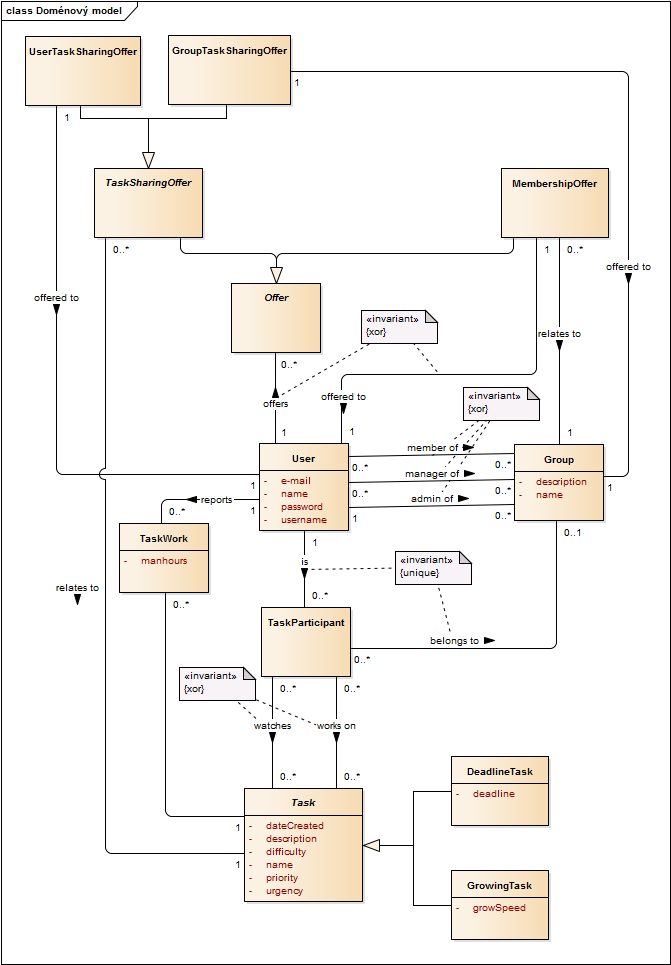
\includegraphics[width=1\textwidth]{ea-diagrams/domain-model.png}
		\caption[Doménový model]{Doménový model aplikace Deadlines}
		\label{diagram:domain-model}
	\end{figure}

\chapter{Detail REST API}
	\label{appdx:restapi}

	\section{Chybové kódy}
		\label{appdx:rest-error-codes}
		\begin{description}
			\item[1] Sometext
			\item[2] Sometext			
		\end{description}
		
		
	\section{Endpointy}
		V této části uvedu pro každý API endpoint detaily o formátu požadavku a odpovědi. Uvedené odpovědi předpokládají, že požadavek proběhl bez chyby. Pokud není uvedeno jinak, HTTP kód odpovědi je 200 OK. V případě chyby při zpracování požadavku aplikace vrací odpovídající chybový HTTP kód a v těle případně detaily chyby, jak jsem popsal v sekci \ref{sec:responses}.
		
		Nepovinná pole v požadavku jsou označena symbolem \texttt{-}.
	
		\subsection{\texttt{GET /user}}
			Formát odpovědi:
			\begin{Verbatim}[obeytabs,tabsize=2]
[
	{
		"id": 1,
		"username": "jdoe",
		-"email": "sample@email.com",
		-"name": "John Doe"
	},
	{
		...
	}
]
			\end{Verbatim}

			
		\subsection{\texttt{POST /user}}
			Formát požadavku:
			\begin{Verbatim}[obeytabs,tabsize=2]
{
	"username": "jdoe",
	"password": "sample-password",
	-"email": "sample@email.com",
	-"name": "John Doe"
}	
			\end{Verbatim}
			
			\noindent
			Formát odpovědi je stejný jako formát požadavku. Při úspěšném vytvoření uživatele je vrácen kód 201 CREATED.
			

		\subsection{\texttt{GET /user/\{user\_id\}}}
			Formát odpovědi:
			\begin{Verbatim}[obeytabs,tabsize=2]
{
	"id": 1,
	"username": "jdoe",
	-"email": "sample@email.com",
	-"name": "John Doe"
}
			\end{Verbatim}
			
		\subsection{\texttt{PUT /user/\{user\_id\}}}
			Formát požadavku:
			\begin{Verbatim}[obeytabs,tabsize=2]			
{
	-"password": "new-password",
	-"email": "new@email.com",
	-"name": "New Doe"
}				
			\end{Verbatim}
			
			\noindent
			Formát odpovědi:
			\begin{Verbatim}[obeytabs,tabsize=2]
{
	"id": 1,
	"username": "jdoe",
	-"email": "new@email.com",
	-"name": "New Doe"
}
			\end{Verbatim}


		\subsection{\texttt{GET /task}}
			Možné parametry:
			\begin{description}
				\item[order] určuje způsob řazení úkolů. Výchozí způsob je podle urgentnosti. Povolené hodnoty jsou: 
				\begin{description}
					\item[name] řazení podle jména;
					\item[date] řazení podle data vytvoření úkolu;
					\item[deadline] řazení podle deadlinu, úkoly bez deadlinu jsou umístěny na konec;
					\item[worked] řazení podle procentuální rozpracovanosti;
					\item[priority] řazení podle priority;
					\item[urgency] řazení podle urgentnosti.
				\end{description}
				
				\item[orderdirection] určuje směr řazení. Výchozí směr je sestupně. Povolené hodnoty jsou:
				\begin{description}
					\item[asc] řazení vzestupně;
					\item[desc] řazení sestupně.
				\end{description}
				
				\item[rolefilter] určuje filtr rolí -- budou zobrazeny pouze úkoly, v nichž má uživatel danou roli. Povolené hodnoty jsou:
				\begin{description}
					\item[watcher] zobrazí jen úkoly, v nichž je uživatel Pozorovatelem;
					\item[worker] zobrazí jen úkoly, v nichž je uživatel Pracovníkem.
				\end{description}
				
				\item[typefilter] určuje filtr podle typu úkolu. Povolené hodnoty jsou:
				\begin{description}
					\item[deadline] zobrazí jen úkoly s deadlinem;
					\item[growing] zobrazí jen rostoucí úkoly.
				\end{description}
				
				\item[statusfilter] určuje filtr podle stavu úkolu. Povolené hodnoty jsou:
				\begin{description}
					\item[open] zobrazí jen úkoly ve stavu \textit{otevřený};
					\item[inprogress] zobrazí jen úkoly ve stavu \textit{rozpracovaný};
					\item[completed] zobrazí jen úkoly ve stavu \textit{splněný};
					\item[cancelled] zobrazí jen úkoly ve stavu \textit{zrušený}.
				\end{description}							
				
				
				\item[priorityfilter] určuje filtr podle priority. Jednotlivé hodnoty lze kombinovat pro zobrazení různých priorit. Povolené hodnoty jsou \textit{lowest}, \textit{low}, \textit{normal}, \textit{high} a \textit{highest}.
			\end{description}
			
			\noindent
			Příklad URL požadavku na tento endpoint, který zobrazí všechny moje úkoly s prioritou 2 nebo 3, seřazené podle rozpracovanosti vzestupně:\\
			\begin{Verbatim}[obeytabs,tabsize=2]
  GET /task?order=worked
           &orderdirection=asc
           &priorityfilter=high
           &priorityfilter=highest
			\end{Verbatim}
			
			\noindent
			Formát odpovědi:
			\begin{Verbatim}[obeytabs,tabsize=2]
[
	{
		"id": 4,
		"name": "Task4",
		"priority": "LOWEST",
		"status": "OPEN",
		"urgency": {
			"lastUpdate": "2016-05-01 16:24",
			"value": 85.31240623606338
		},
		"deadline": "2016-05-02 02:24",
		"workedPercentage": 0.0,
		"type": "DEADLINE"
	},
	{
		...
	}
]
			\end{Verbatim}
			
			
		\subsection{\texttt{POST /task}}
			Formát požadavku:
			\begin{Verbatim}[obeytabs,tabsize=2]
{
	"name": "task name",
	"description":"task description",
	"priority": "LOW",
	"workEstimate": "13",
	"deadline":"2016-05-17 13:15",
	"hoursToPeak":"3",
	"groupIds":"1,3,8"
}
			\end{Verbatim}
			Požadavek musí mít vyplněno právě jedno z polí \texttt{deadline} a \texttt{hoursToPeak}. Podle nich se určí typ vytvořeného úkolu.
			
			Pole \texttt{groupIds} může obsahovat ID skupin, v nichž je volající uživatel manažer. Úkol bude po vytvoření automaticky sdílen s těmito skupinami.
			
			\hfill \\
			\noindent
			Formát odpovědi:
			\begin{Verbatim}[obeytabs,tabsize=2]
{
	"id": 2,
	"dateCreated": "2016-05-01 16:11",
	"name": "task name",
	"description": "task description",
	"workEstimate": 13.0,
	"priority": "LOW",
	"status": "OPEN",
	"urgency": {
		"lastUpdate": "2016-05-01 16:11",
		"value": 0.0
	},
	"workReports": [],
	"participants": [
		{
			"solo": true,
			"role": "WATCHER",
			"user": {
				"id": 1,
				"username": "User1"
			}
		}
	],
	"hoursToPeak": 12.5 |or| "deadline": "2016-05-17 12:00",
	"workedPercentage": 0.0,
	"manhoursWorked": 0.0,
	"groups": [
		{
			"id": 1,
			"name": "Group1"
		},
		{
			"id": 2,
			"name": "Group4"
		}
	],
	"type": "GROWING"
}
			\end{Verbatim}			
			
			V tomto příkladu je úkol s ID 2 sdílen s jedním uživatelem (\textit{User1}), který je v roli pozorovatele, a se dvěma skupinami (\textit{Group1}, \textit{Group4}).
			
			Při úspěšném vytvoření úkolu je vrácen kód 201 CREATED.
			
			
		\subsection{\texttt{GET /task/\{task\_id\}}}
		\subsection{\texttt{PUT /task/\{task\_id\}}}
		\subsection{\texttt{POST /task/\{task\_id\}/reseturgency}}
		\subsection{\texttt{POST /task/share/\{task\_id\}}}
		\subsection{\texttt{POST /task/leave/\{task\_id\}}}
		\subsection{\texttt{POST /task/role/\{task\_id\}}}
		\subsection{\texttt{POST /task/report/\{task\_id\}}}
		\subsection{\texttt{GET /offer/task/user}}
		\subsection{\texttt{POST /offer/task/user/resolve/\{task\_offer\_id\}}}
		\subsection{\texttt{GET /offer/task/group/\{group\_id\}}}
		\subsection{\texttt{POST /offer/task/group/\{group\_id\}/resolve/\{task\_offer\_id\}}}
		\subsection{\texttt{GET /offer/membership}}
		\subsection{\texttt{POST /offer/membership/resolve/\{membership\_offer\_id\}}}
		\subsection{\texttt{GET /group}}
		\subsection{\texttt{POST /group}}
		\subsection{\texttt{GET /group/\{group\_id\}}}
		\subsection{\texttt{PUT /group/\{group\_id\}}}
		\subsection{\texttt{DELETE /group/\{group\_id\}}}
		\subsection{\texttt{POST /group/\{group\_id\}/member/offer}}
		\subsection{\texttt{PUT /group/\{group\_id\}}/member/\{member\_id\}}
		\subsection{\texttt{DELETE /group/\{group\_id\}}/member/\{member\_id\}}
		\subsection{\texttt{DELETE /group/\{group\_id\}/task/\{task\_id\}}}
		
		
			
			
			
			
			
			
			
			
			
			
				\begin{description}
					\item[]
				\end{description}			

\chapter{Komponenty aplikace}
	\begin{figure}\centering
		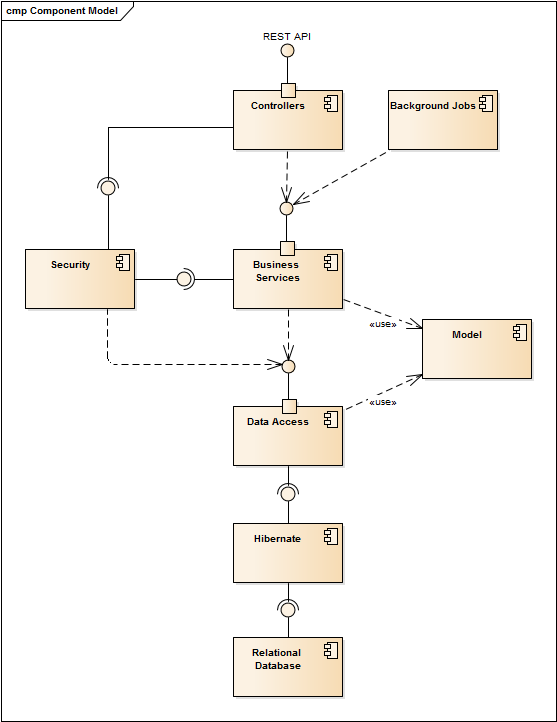
\includegraphics[width=1\textwidth]{ea-diagrams/architecture-diagram.png}
		\caption[Diagram komponent]{Diagram architektury komponent aplikace}
		\label{diagram:component-model}
	\end{figure}

\chapter{Návrhový model}

\begin{figure}\centering
	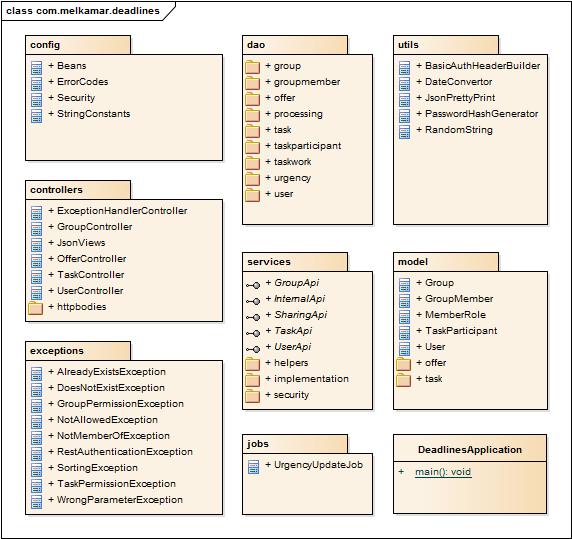
\includegraphics[width=1\textwidth]{ea-diagrams/packages/root.png}
	\caption[Balíčky tříd]{Balíčky a třídy aplikace Deadlines}
	\label{diagram:packages-root}
\end{figure}

\begin{figure}\centering
	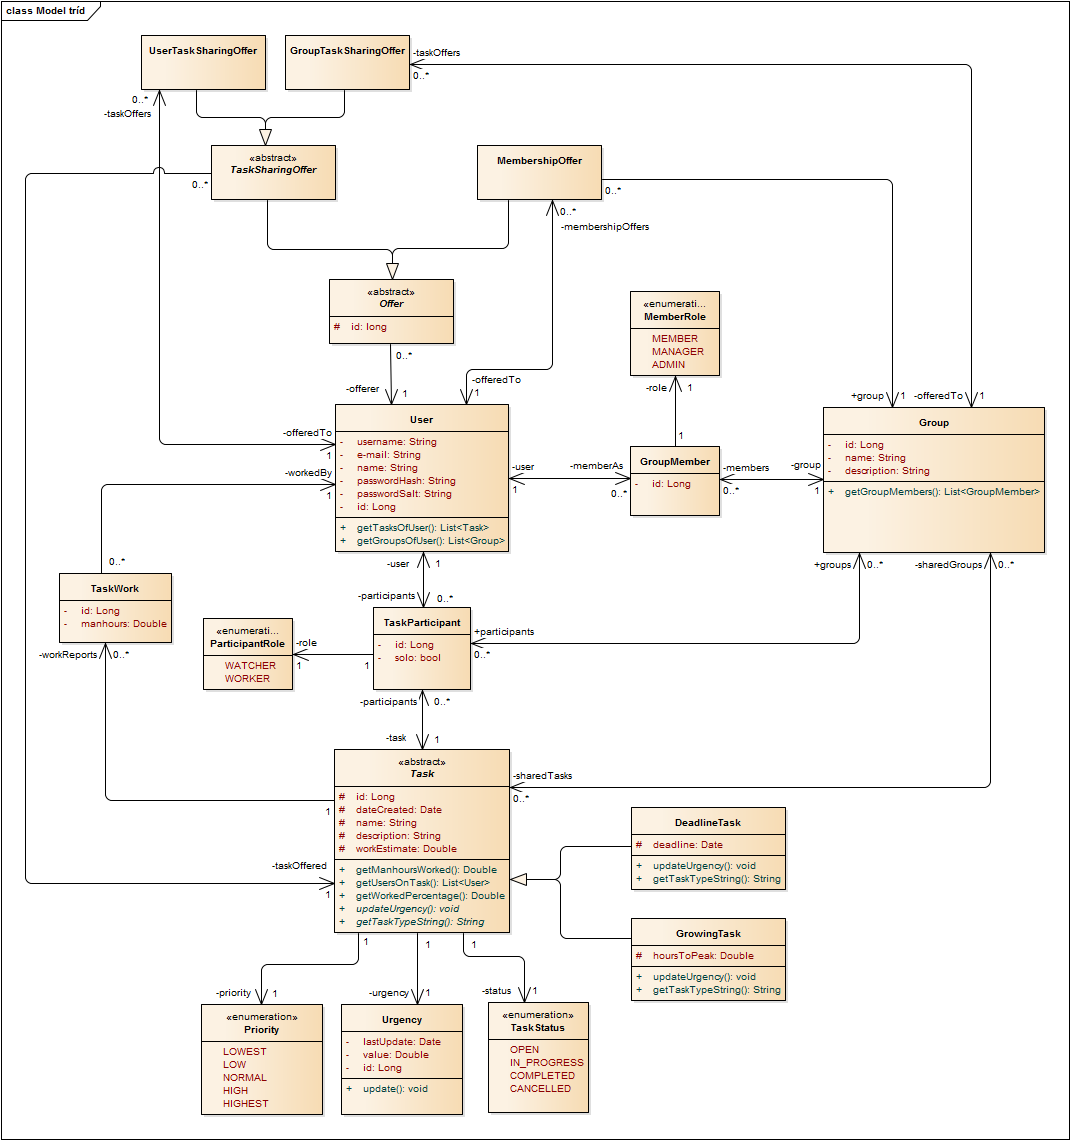
\includegraphics[width=1\textwidth]{ea-diagrams/class-model.png}
	\caption[Model tříd]{Návrhový model tříd aplikace Deadlines}
	\label{diagram:class-model}
\end{figure}

\chapter{Databázový model}
\begin{figure}\centering
	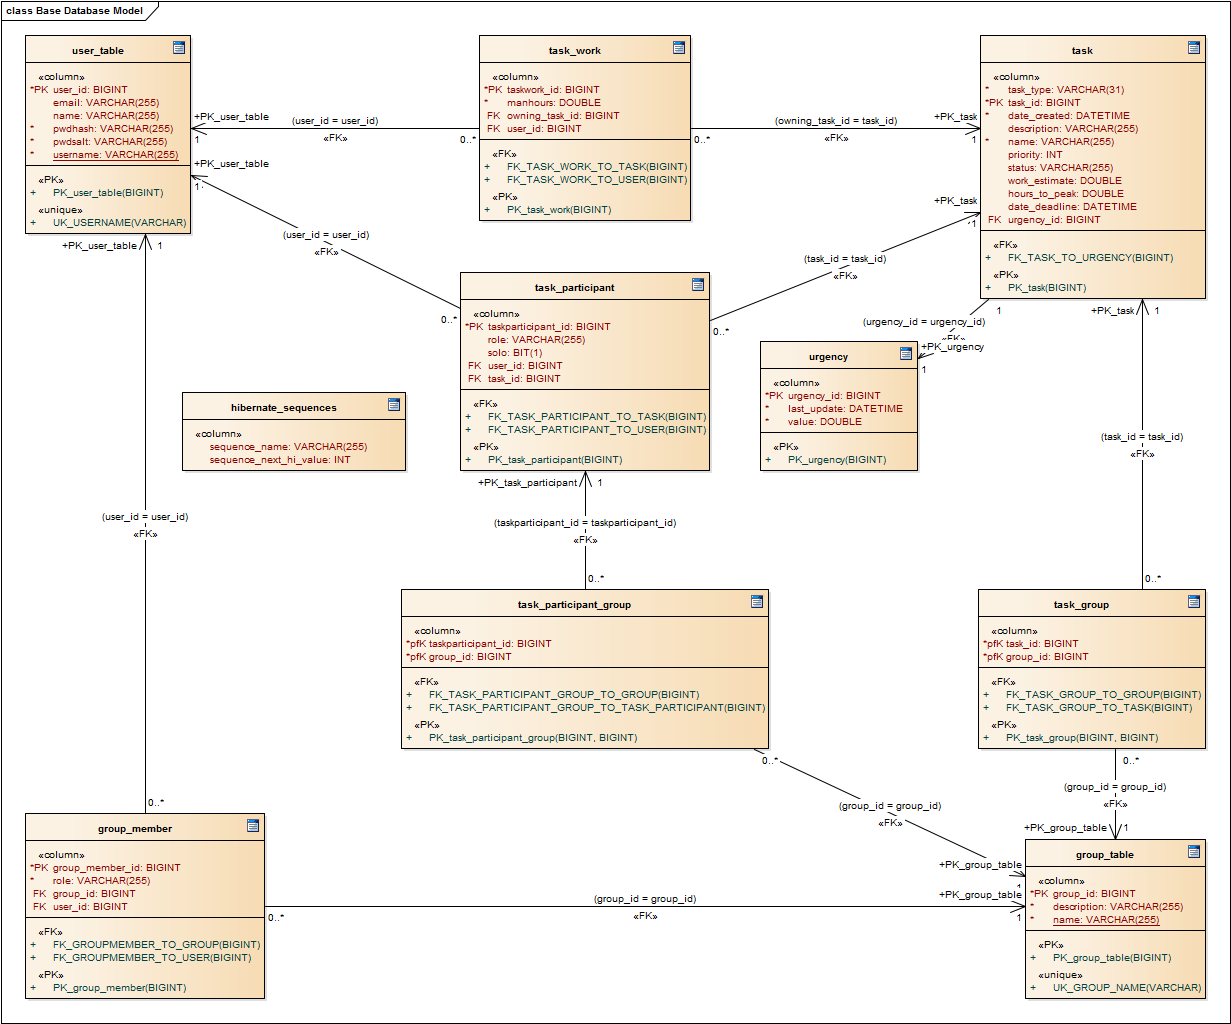
\includegraphics[width=1\textwidth]{ea-diagrams/database/base.png}
	\caption[Databázový model]{Relační databázový model entit aplikace, kromě nabídek}
	\label{diagram:database-model-base}
\end{figure}

\begin{figure}\centering
	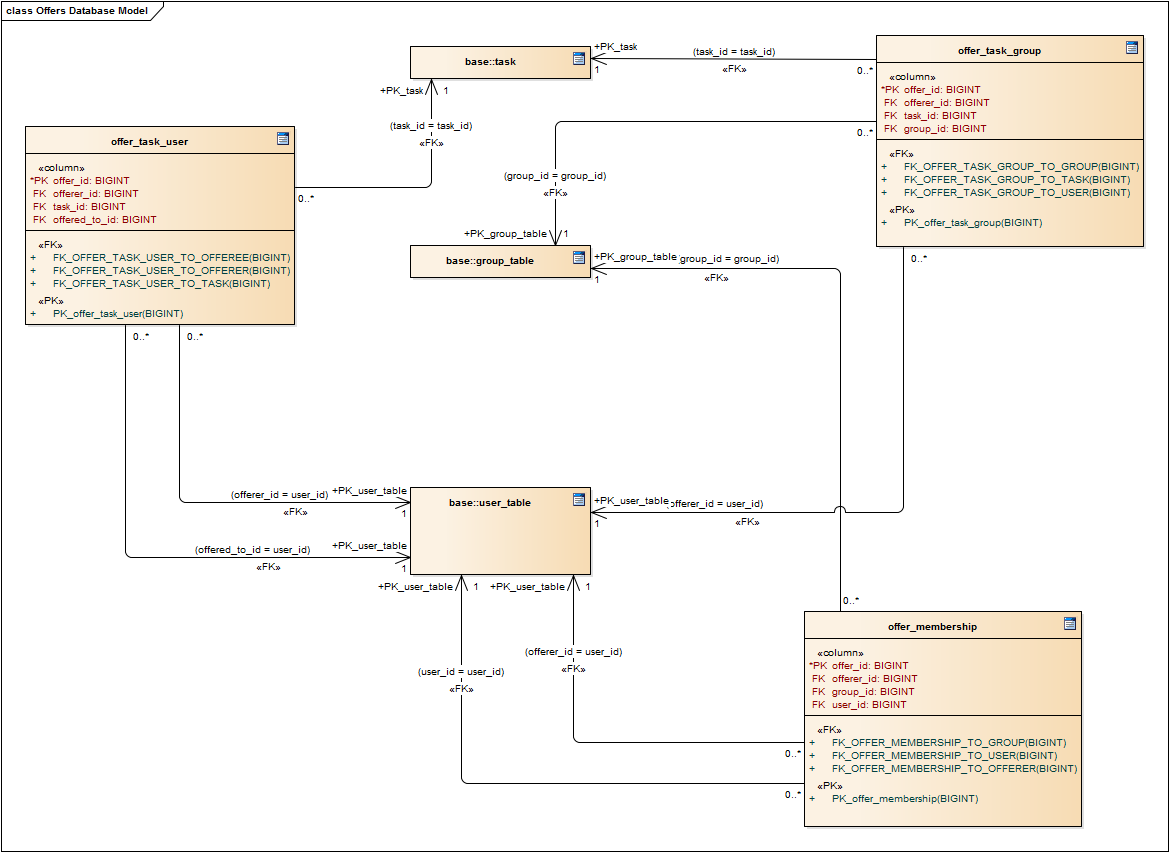
\includegraphics[width=1\textwidth]{ea-diagrams/database/offers.png}
	\caption[Databázový model nabídek]{Relační databázový model nabídek}
	\label{diagram:database-model-offers}
\end{figure}




\chapter{Obsah přiloženého CD}

%upravte podle skutecnosti

\begin{figure}
	\dirtree{%
		.1 readme.txt\DTcomment{stručný popis obsahu CD}.
		.1 exe\DTcomment{adresář se spustitelnou formou implementace}.
		.1 src.
		.2 impl\DTcomment{zdrojové kódy implementace}.
		.2 thesis\DTcomment{zdrojová forma práce ve formátu \LaTeX{}}.
		.1 text\DTcomment{text práce}.
		.2 thesis.pdf\DTcomment{text práce ve formátu PDF}.
		.2 thesis.ps\DTcomment{text práce ve formátu PS}.
	}
\end{figure}

\end{document}

% % % % % % % % % % % % % % % % % % % % % % % % % % % % 
% % Tuto kapitolu z výsledné práce ODSTRAŇTE.
% % % % % % % % % % % % % % % % % % % % % % % % % % % % 
% 
% \chapter{Návod k~použití této šablony}
% 
% Tento dokument slouží jako základ pro napsání závěrečné práce na Fakultě informačních technologií ČVUT v~Praze.
% 
% \section{Výběr základu}
% 
% Vyberte si šablonu podle druhu práce (bakalářská, diplomová), jazyka (čeština, angličtina) a kódování (ASCII, \mbox{UTF-8}, \mbox{ISO-8859-2} neboli latin2 a nebo \mbox{Windows-1250}). 
% 
% V~české variantě naleznete šablony v~souborech pojmenovaných ve formátu práce\_kódování.tex. Typ může být:
% \begin{description}
% 	\item[BP] bakalářská práce,
% 	\item[DP] diplomová (magisterská) práce.
% \end{description}
% Kódování, ve kterém chcete psát, může být:
% \begin{description}
% 	\item[UTF-8] kódování Unicode,
% 	\item[ISO-8859-2] latin2,
% 	\item[Windows-1250] znaková sada 1250 Windows.
% \end{description}
% V~případě nejistoty ohledně kódování doporučujeme následující postup:
% \begin{enumerate}
% 	\item Otevřete šablony pro kódování UTF-8 v~editoru prostého textu, který chcete pro psaní práce použít -- pokud můžete texty s~diakritikou normálně přečíst, použijte tuto šablonu.
% 	\item V~opačném případě postupujte dále podle toho, jaký operační systém používáte:
% 	\begin{itemize}
% 		\item v~případě Windows použijte šablonu pro kódování \mbox{Windows-1250},
% 		\item jinak zkuste použít šablonu pro kódování \mbox{ISO-8859-2}.
% 	\end{itemize}
% \end{enumerate}
% 
% 
% V~anglické variantě jsou šablony pojmenované podle typu práce, možnosti jsou:
% \begin{description}
% 	\item[bachelors] bakalářská práce,
% 	\item[masters] diplomová (magisterská) práce.
% \end{description}
% 
% \section{Použití šablony}
% 
% Šablona je určena pro zpracování systémem \LaTeXe{}. Text je možné psát v~textovém editoru jako prostý text, lze však také využít specializovaný editor pro \LaTeX{}, např. Kile.
% 
% Pro získání tisknutelného výstupu z~takto vytvořeného souboru použijte příkaz \verb|pdflatex|, kterému předáte cestu k~souboru jako parametr. Vhodný editor pro \LaTeX{} toto udělá za Vás. \verb|pdfcslatex| ani \verb|cslatex| \emph{nebudou} s~těmito šablonami fungovat.
% 
% Více informací o~použití systému \LaTeX{} najdete např. v~\cite{wikilatex}.
% 
% \subsection{Typografie}
% 
% Při psaní dodržujte typografické konvence zvoleného jazyka. České \uv{uvozovky} zapisujte použitím příkazu \verb|\uv|, kterému v~parametru předáte text, jenž má být v~uvozovkách. Anglické otevírací uvozovky se v~\LaTeX{}u zadávají jako dva zpětné apostrofy, uzavírací uvozovky jako dva apostrofy. Často chybně uváděný symbol "{} (palce) nemá s~uvozovkami nic společného.
% 
% Dále je třeba zabránit zalomení řádky mezi některými slovy, v~češtině např. za jednopísmennými předložkami a spojkami (vyjma \uv{a}). To docílíte vložením pružné nezalomitelné mezery -- znakem \texttt{\textasciitilde}. V~tomto případě to není třeba dělat ručně, lze použít program \verb|vlna|.
% 
% Více o~typografii viz \cite{kobltypo}.
% 
% \subsection{Obrázky}
% 
% Pro umožnění vkládání obrázků je vhodné použít balíček \verb|graphicx|, samotné vložení se provede příkazem \verb|\includegraphics|. Takto je možné vkládat obrázky ve formátu PDF, PNG a JPEG jestliže používáte pdf\LaTeX{} nebo ve formátu EPS jestliže používáte \LaTeX{}. Doporučujeme preferovat vektorové obrázky před rastrovými (vyjma fotografií).
% 
% \subsubsection{Získání vhodného formátu}
% 
% Pro získání vektorových formátů PDF nebo EPS z~jiných lze použít některý z~vektorových grafických editorů. Pro převod rastrového obrázku na vektorový lze použít rasterizaci, kterou mnohé editory zvládají (např. Inkscape). Pro konverze lze použít též nástroje pro dávkové zpracování běžně dodávané s~\LaTeX{}em, např. \verb|epstopdf|.
% 
% \subsubsection{Plovoucí prostředí}
% 
% Příkazem \verb|\includegraphics| lze obrázky vkládat přímo, doporučujeme však použít plovoucí prostředí, konkrétně \verb|figure|. Například obrázek \ref{fig:float} byl vložen tímto způsobem. Vůbec přitom nevadí, když je obrázek umístěn jinde, než bylo původně zamýšleno -- je tomu tak hlavně kvůli dodržení typografických konvencí. Namísto vynucování konkrétní pozice obrázku doporučujeme používat odkazování z~textu (dvojice příkazů \verb|\label| a \verb|\ref|).
% 
% \begin{figure}\centering
% 	
\includegraphics[width=0.5\textwidth, angle=30]{cvut-logo-bw}
% 	\caption[Příklad obrázku]{Ukázkový obrázek v~plovoucím prostředí}\label{fig:float}
% \end{figure}
% 
% \subsubsection{Verze obrázků}
% 
% % Gnuplot BW i barevně
% Může se hodit mít více verzí stejného obrázku, např. pro barevný či černobílý tisk a nebo pro prezentaci. S~pomocí některých nástrojů na generování grafiky je to snadné.
% 
% Máte-li například graf vytvořený v programu Gnuplot, můžete jeho černobílou variantu (viz obr. \ref{fig:gnuplot-bw}) vytvořit parametrem \verb|monochrome dashed| příkazu \verb|set term|. Barevnou variantu (viz obr. \ref{fig:gnuplot-col}) vhodnou na prezentace lze vytvořit parametrem \verb|colour solid|.
% 
% \begin{figure}\centering
% 	\includegraphics{gnuplot-bw}
% 	\caption{Černobílá varianta obrázku generovaného programem Gnuplot}\label{fig:gnuplot-bw}
% \end{figure}
% 
% \begin{figure}\centering
% 	\includegraphics{gnuplot-col}
% 	\caption{Barevná varianta obrázku generovaného programem Gnuplot}\label{fig:gnuplot-col}
% \end{figure}
% 
% 
% \subsection{Tabulky}
% 
% Tabulky lze zadávat různě, např. v~prostředí \verb|tabular|, avšak pro jejich vkládání platí to samé, co pro obrázky -- použijte plovoucí prostředí, v~tomto případě \verb|table|. Například tabulka \ref{tab:matematika} byla vložena tímto způsobem.
% 
% \begin{table}\centering
% 	\caption[Příklad tabulky]{Zadávání matematiky}\label{tab:matematika}
% 	\begin{tabular}{|l|l|c|c|}\hline
% 		Typ		& Prostředí		& \LaTeX{}ovská zkratka	& \TeX{}ovská zkratka	\tabularnewline \hline \hline
% 		Text		& \verb|math|		& \verb|\(...\)|	& \verb|$...$|		\tabularnewline \hline
% 		Displayed	& \verb|displaymath|	& \verb|\[...\]|	& \verb|$$...$$|	\tabularnewline \hline
% 	\end{tabular}
% \end{table}
% 
% % % % % % % % % % % % % % % % % % % % % % % % % % % % 